\documentclass[a4paper,pagesize,12pt,bibtotoc,pointlessnumbers,
normalheadings,DIV=11,twoside=false]{scrbook}

% twoside, openright
\KOMAoptions{DIV=last}

\usepackage{trajan}
 
\usepackage[portuguese]{babel}
\usepackage[utf8]{inputenc}
\usepackage[T1]{fontenc}
\usepackage{graphicx}
\usepackage{float}
\usepackage[sc]{mathpazo}
\linespread{1.05} 
\usepackage{verbatim} % for comments
\usepackage{listings} % for comments
\usepackage{indentfirst}
\usepackage{gensymb}
\usepackage{hyperref}
\usepackage{multirow}
\usepackage{enumerate}
\usepackage{subfigure}
\usepackage{array}
\usepackage{varwidth}
\usepackage{imakeidx}
\makeindex
\usepackage{blindtext}
%%%%%%%%%%%%%%%%%%%%%%%%%%%%%%%%%%%%%%%%%
% This is based on the Legrand Orange Book
% Structural Definitions File
%
% The original template (the Legrand Orange Book Template) can be found here --> http://www.latextemplates.com/template/the-legrand-orange-book
%
% Original author of the Legrand Orange Book Template::
% Mathias Legrand (legrand.mathias@gmail.com) with modifications by:
% Vel (vel@latextemplates.com)
%
% Original License:
% CC BY-NC-SA 3.0 (http://creativecommons.org/licenses/by-nc-sa/3.0/)
%
%%%%%%%%%%%%%%%%%%%%%%%%%%%%%%%%%%%%%%%%%
%----------------------------------------------------------------------------------------
%	VARIOUS REQUIRED PACKAGES
%----------------------------------------------------------------------------------------

\usepackage{titlesec} % Allows customization of titles

\usepackage{graphicx} % Required for including pictures
\graphicspath{{Pictures/}} % Specifies the directory where pictures are stored

\usepackage{lipsum} % Inserts dummy text

\usepackage{tikz} % Required for drawing custom shapes

\usepackage[portuguese]{babel} 

\usepackage{enumitem} % Customize lists

\setlist{nolistsep} % Reduce spacing between bullet points and numbered lists

\usepackage{booktabs} % Required for nicer horizontal rules in tables

\usepackage{eso-pic} % Required for specifying an image background in the title page

\usepackage{glossaries} %Required to allow the creation of glossary items, allows for referencing within the document

\usepackage[none]{hyphenat} %Stops words which are too long for a line being split over two lines using hyphenation

\usepackage[top=3cm,bottom=3cm,left=3.2cm,right=3.2cm,headsep=5pt,letterpaper]{geometry} % Page margins
\usepackage{algorithm} % Writing nice algorithms
\usepackage{algpseudocode} % Writing pseudocode
\usepackage{longtable} %Tables which may stretch over more than 1 page
\usepackage{rotating} %Rotate images using sideswaysimage


% Font Settings
\usepackage{forum} % Use the Avantgarde font for headings
%\usepackage{times} % Use the Times font for headings
\usepackage{mathptmx} % Use the Adobe Times Roman as the default text font together with math symbols from the Symbol, Chancery and Computer Modern fonts

\usepackage{microtype} % Slightly tweak font spacing for aesthetics
\usepackage[utf8]{inputenc} % Required for including letters with accents
\usepackage[T1]{fontenc} % Use 8-bit encoding that has 256 glyphs


%----------------------------------------------------------------------------------------
%	MAIN TABLE OF CONTENTS
%----------------------------------------------------------------------------------------

\usepackage{titletoc} % Required for manipulating the table of contents

\contentsmargin{0cm} % Removes the default margin
% Chapter text styling
\titlecontents{chapter}[1.25cm] % Indentation
{\addvspace{10pt}\large\sffamily\bfseries} % Spacing and font options for chapters
{\color{Apricot!60}\contentslabel[\Large\thecontentslabel]{1.25cm}\color{Apricot}} % Chapter number
{}  
{\color{Apricot!60}\normalsize\sffamily\bfseries\;\titlerule*[.5pc]{.}\;\thecontentspage} % Page number
% Section text styling
\titlecontents{section}[1.25cm] % Indentation
{\addvspace{5pt}\sffamily\bfseries} % Spacing and font options for sections
{\contentslabel[\thecontentslabel]{1.25cm}} % Section number
{}
{\sffamily\;\titlerule*[.5pc]{.}\;\thecontentspage} % Page number
[]
% Subsection text styling
\titlecontents{subsection}[1.25cm] % Indentation
{\addvspace{1pt}\sffamily} % Spacing and font options for subsections
{\contentslabel[\thecontentslabel]{1.25cm}} % Subsection number
{}
{\sffamily\;\titlerule*[.5pc]{.}\;\thecontentspage} % Page number
[] 

%----------------------------------------------------------------------------------------
%	MINI TABLE OF CONTENTS IN CHAPTER HEADS
%----------------------------------------------------------------------------------------

% Section text styling
\titlecontents{lsection}[0em] % Indendating
{\footnotesize\sffamily} % Font settings
{}
{}
{}

% Subsection text styling
\titlecontents{lsubsection}[.5em] % Indentation
{\normalfont\footnotesize\sffamily} % Font settings
{}
{}
{}
 
%----------------------------------------------------------------------------------------
%	PAGE HEADERS
%----------------------------------------------------------------------------------------

\usepackage{fancyhdr} % Required for header and footer configuration

\pagestyle{fancy}
\renewcommand{\chaptermark}[1]{\markboth{\sffamily\normalsize\bfseries\chaptername\ \thechapter.\ #1}{}} % Chapter text font settings
\renewcommand{\sectionmark}[1]{\markright{\sffamily\normalsize\thesection\hspace{10pt}#1}{}} % Section text font settings
\fancyhf{} \fancyhead[LE,RO]{\sffamily\normalsize\thepage} % Font setting for the page number in the header
\fancyhead[LO]{\rightmark} % Print the nearest section name on the left side of odd pages
\fancyhead[RE]{\leftmark} % Print the current chapter name on the right side of even pages
\renewcommand{\headrulewidth}{0.5pt} % Width of the rule under the header
\addtolength{\headheight}{2.5pt} % Increase the spacing around the header slightly
\renewcommand{\footrulewidth}{0pt} % Removes the rule in the footer
\fancypagestyle{plain}{\fancyhead{}\renewcommand{\headrulewidth}{0pt}} % Style for when a plain pagestyle is specified

% Removes the header from odd empty pages at the end of chapters
\makeatletter
\renewcommand{\cleardoublepage}{
\clearpage\ifodd\c@page\else
\hbox{}
\vspace*{\fill}
\thispagestyle{empty}
\newpage
\fi}

%----------------------------------------------------------------------------------------
%	THEOREM STYLES
%----------------------------------------------------------------------------------------

\usepackage{amsmath,amsfonts,amssymb,amsthm} % For math equations, theorems, symbols, etc

\newcommand{\intoo}[2]{\mathopen{]}#1\,;#2\mathclose{[}}
\newcommand{\ud}{\mathop{\mathrm{{}d}}\mathopen{}}
\newcommand{\intff}[2]{\mathopen{[}#1\,;#2\mathclose{]}}
\newtheorem{notation}{Notation}[chapter]

%%%%%%%%%%%%%%%%%%%%%%%%%%%%%%%%%%%%%%%%%%%%%%%%%%%%%%%%%%%%%%%%%%%%%%%%%%%
%%%%%%%%%%%%%%%%%%%% dedicated to boxed/framed environements %%%%%%%%%%%%%%
%%%%%%%%%%%%%%%%%%%%%%%%%%%%%%%%%%%%%%%%%%%%%%%%%%%%%%%%%%%%%%%%%%%%%%%%%%%
\newtheoremstyle{Orchidnumbox}% % Theorem style name
{0pt}% Space above
{0pt}% Space below
{\normalfont}% % Body font
{}% Indent amount
{\small\bf\sffamily\color{Apricot}}% % Theorem head font
{\;}% Punctuation after theorem head
{0.25em}% Space after theorem head
{\small\sffamily\color{Apricot}\thmname{#1}\nobreakspace\thmnumber{\@ifnotempty{#1}{}\@upn{#2}}% Theorem text (e.g. Theorem 2.1)
\thmnote{\nobreakspace\the\thm@notefont\sffamily\bfseries\color{black}---\nobreakspace#3.}} % Optional theorem note
\renewcommand{\qedsymbol}{$\blacksquare$}% Optional qed square

\newtheoremstyle{blacknumex}% Theorem style name
{5pt}% Space above
{5pt}% Space below
{\normalfont}% Body font
{} % Indent amount
{\small\bf\sffamily}% Theorem head font
{\;}% Punctuation after theorem head
{0.25em}% Space after theorem head
{\small\sffamily{\tiny\ensuremath{\blacksquare}}\nobreakspace\thmname{#1}\nobreakspace\thmnumber{\@ifnotempty{#1}{}\@upn{#2}}% Theorem text (e.g. Theorem 2.1)
\thmnote{\nobreakspace\the\thm@notefont\sffamily\bfseries---\nobreakspace#3.}}% Optional theorem note

\newtheoremstyle{blacknumbox} % Theorem style name
{0pt}% Space above
{0pt}% Space below
{\normalfont}% Body font
{}% Indent amount
{\small\bf\sffamily}% Theorem head font
{\;}% Punctuation after theorem head
{0.25em}% Space after theorem head
{\small\sffamily\thmname{#1}\nobreakspace\thmnumber{\@ifnotempty{#1}{}\@upn{#2}}% Theorem text (e.g. Theorem 2.1)
\thmnote{\nobreakspace\the\thm@notefont\sffamily\bfseries---\nobreakspace#3.}}% Optional theorem note

%%%%%%%%%%%%%%%%%%%%%%%%%%%%%%%%%%%%%%%%%%%%%%%%%%%%%%%%%%%%%%%%%%%%%%%%%%%
%%%%%%%%%%%%% dedicated to non-boxed/non-framed environements %%%%%%%%%%%%%
%%%%%%%%%%%%%%%%%%%%%%%%%%%%%%%%%%%%%%%%%%%%%%%%%%%%%%%%%%%%%%%%%%%%%%%%%%%
\newtheoremstyle{Orchidnum}% % Theorem style name
{5pt}% Space above
{5pt}% Space below
{\normalfont}% % Body font
{}% Indent amount
{\small\bf\sffamily\color{Apricot}}% % Theorem head font
{\;}% Punctuation after theorem head
{0.25em}% Space after theorem head
{\small\sffamily\color{Apricot}\thmname{#1}\nobreakspace\thmnumber{\@ifnotempty{#1}{}\@upn{#2}}% Theorem text (e.g. Theorem 2.1)
\thmnote{\nobreakspace\the\thm@notefont\sffamily\bfseries\color{black}---\nobreakspace#3.}} % Optional theorem note
\renewcommand{\qedsymbol}{$\blacksquare$}% Optional qed square
\makeatother

% Defines the theorem text style for each type of theorem to one of the three styles above
\newcounter{dummy} 
\numberwithin{dummy}{section}
\theoremstyle{Orchidnumbox}
\newtheorem{theoremeT}[dummy]{Theorem}
\newtheorem{problem}{Problem}[chapter]
\newtheorem{exerciseT}{Exercise}[chapter]
\theoremstyle{blacknumex}
\newtheorem{exampleT}{Example}[chapter]
\theoremstyle{blacknumbox}
\newtheorem{vocabulary}{Vocabulary}[chapter]
\newtheorem{definitionT}{Definition}[section]
\newtheorem{corollaryT}[dummy]{Corollary}
\theoremstyle{Orchidnum}
\newtheorem{proposition}[dummy]{Proposition}

%----------------------------------------------------------------------------------------
%	DEFINITION OF COLORED BOXES
%----------------------------------------------------------------------------------------

\RequirePackage[framemethod=default]{mdframed} % Required for creating the theorem, definition, exercise and corollary boxes

% Theorem box
\newmdenv[skipabove=7pt,
skipbelow=7pt,
backgroundcolor=black!5,
linecolor= Apricot, % Modify the colour of theorem boxes
innerleftmargin=5pt,
innerrightmargin=5pt,
innertopmargin=5pt,
leftmargin=0cm,
rightmargin=0cm,
innerbottommargin=5pt]{tBox}

% Exercise box	  
\newmdenv[skipabove=7pt,
skipbelow=7pt,
rightline=false,
leftline=true,
topline=false,
bottomline=false,
backgroundcolor=Apricot!10,
linecolor=Apricot,
innerleftmargin=5pt,
innerrightmargin=5pt,
innertopmargin=5pt,
innerbottommargin=5pt,
leftmargin=0cm,
rightmargin=0cm,
linewidth=4pt]{eBox}	

% Definition box
\newmdenv[skipabove=7pt,
skipbelow=7pt,
rightline=false,
leftline=true,
topline=false,
bottomline=false,
linecolor=Apricot,
innerleftmargin=5pt,
innerrightmargin=5pt,
innertopmargin=0pt,
leftmargin=0cm,
rightmargin=0cm,
linewidth=4pt,
innerbottommargin=0pt]{dBox}	

% Corollary box
\newmdenv[skipabove=7pt,
skipbelow=7pt,
rightline=false,
leftline=true,
topline=false,
bottomline=false,
linecolor=gray,
backgroundcolor=black!5,
innerleftmargin=5pt,
innerrightmargin=5pt,
innertopmargin=5pt,
leftmargin=0cm,
rightmargin=0cm,
linewidth=4pt,
innerbottommargin=5pt]{cBox}

% Creates an environment for each type of theorem and assigns it a theorem text style from the "Theorem Styles" section above and a colored box from above
\newenvironment{theorem}{\begin{tBox}\begin{theoremeT}}{\end{theoremeT}\end{tBox}}
\newenvironment{exercise}{\begin{eBox}\begin{exerciseT}}{\hfill{\color{Apricot}\tiny\ensuremath{\blacksquare}}\end{exerciseT}\end{eBox}}				  
\newenvironment{definition}{\begin{dBox}\begin{definitionT}}{\end{definitionT}\end{dBox}}	
\newenvironment{example}{\begin{exampleT}}{\hfill{\tiny\ensuremath{\blacksquare}}\end{exampleT}}		
\newenvironment{corollary}{\begin{cBox}\begin{corollaryT}}{\end{corollaryT}\end{cBox}}	

%----------------------------------------------------------------------------------------
%	REMARK ENVIRONMENT
%----------------------------------------------------------------------------------------

\newenvironment{remark}{\par\vspace{10pt}\small % Vertical white space above the remark and smaller font size
\begin{list}{}{
\leftmargin=35pt % Indentation on the left
\rightmargin=25pt}\item\ignorespaces % Indentation on the right
\makebox[-2.5pt]{\begin{tikzpicture}[overlay]
\node[draw=Orchid!60,line width=1pt,circle,fill=Orchid!25,font=\sffamily\bfseries,inner sep=2pt,outer sep=0pt] at (-15pt,0pt){\textcolor{Apricot}{R}};\end{tikzpicture}} % Orange R in a circle
\advance\baselineskip -1pt}{\end{list}\vskip5pt} % Tighter line spacing and white space after remark

%----------------------------------------------------------------------------------------
%	SECTION NUMBERING IN THE MARGIN
%----------------------------------------------------------------------------------------

\makeatletter
\renewcommand{\@seccntformat}[1]{\llap{\textcolor{Apricot}{\csname the#1\endcsname}\hspace{1em}}}                    
\renewcommand{\section}{\@startsection{section}{1}{\z@}
{-4ex \@plus -1ex \@minus -.4ex}
{1ex \@plus.2ex }
{\normalfont\large\sffamily\bfseries}}
\renewcommand{\subsection}{\@startsection {subsection}{2}{\z@}
{-3ex \@plus -0.1ex \@minus -.4ex}
{0.5ex \@plus.2ex }
{\normalfont\sffamily\bfseries}}
\renewcommand{\subsubsection}{\@startsection {subsubsection}{3}{\z@}
{-2ex \@plus -0.1ex \@minus -.2ex}
{.2ex \@plus.2ex }
{\normalfont\small\sffamily\bfseries}}                        
\renewcommand\paragraph{\@startsection{paragraph}{4}{\z@}
{-2ex \@plus-.2ex \@minus .2ex}
{.1ex}
{\normalfont\small\sffamily\bfseries}}

%----------------------------------------------------------------------------------------
%	HYPERLINKS IN THE DOCUMENTS
%----------------------------------------------------------------------------------------

% For an unclear reason, the package should be loaded now and not later
\usepackage{hyperref}
\hypersetup{hidelinks,colorlinks=false,breaklinks=true,urlcolor= Orchid,bookmarksopen=false,pdftitle={Title},pdfauthor={Author}}

%----------------------------------------------------------------------------------------
%	CHAPTER HEADINGS
%----------------------------------------------------------------------------------------

% The set-up below should be (sadly) manually adapted to the overall margin page septup controlled by the geometry package loaded in the main.tex document. It is possible to implement below the dimensions used in the goemetry package (top,bottom,left,right)... TO BE DONE

\newcommand{\thechapterimage}{}
\newcommand{\chapterimage}[1]{\renewcommand{\thechapterimage}{#1}}

% Numbered chapters with mini tableofcontents
\def\thechapter{\arabic{chapter}}
\def\@makechapterhead#1{
\thispagestyle{empty}
{\centering \normalfont\sffamily
\ifnum \c@secnumdepth >\m@ne
\if@mainmatter
\startcontents
\begin{tikzpicture}[remember picture,overlay]
\node at (current page.north west)
{\begin{tikzpicture}[remember picture,overlay]
\node[anchor=north west,inner sep=0pt] at (0,0) {\includegraphics[width=\paperwidth]{\thechapterimage}};
%%%%%%%%%%%%%%%%%%%%%%%%%%%%%%%%%%%%%%%%%%%%%%%%%%%%%%%%%%%%%%%%%%%%%%%%%%%%%%%%%%%%%
% Commenting the 3 lines below removes the small contents box in the chapter heading
%\fill[color=Orchid!10!white,opacity=.6] (1cm,0) rectangle (8cm,-7cm);
%\node[anchor=north west] at (1.1cm,.35cm) {\parbox[t][8cm][t]{6.5cm}{\huge\bfseries\flushleft \printcontents{l}{1}{\setcounter{tocdepth}{2}}}};
\draw[anchor=west] (3cm,-4.5cm) node [rounded corners=20pt,fill=Apricot!10!white,text opacity=1,draw=Apricot,draw opacity=1,line width=1.5pt,fill opacity=.6,inner sep=12pt]{\huge\sffamily\bfseries\textcolor{black}{\thechapter. #1\strut\makebox[22cm]{}}};
%%%%%%%%%%%%%%%%%%%%%%%%%%%%%%%%%%%%%%%%%%%%%%%%%%%%%%%%%%%%%%%%%%%%%%%%%%%%%%%%%%%%%
\end{tikzpicture}};
\end{tikzpicture}}
\par\vspace*{70\p@}
\fi
\fi}

% Unnumbered chapters without mini tableofcontents (could be added though) 
\def\@makeschapterhead#1{
\thispagestyle{empty}
{\centering \normalfont\sffamily
\ifnum \c@secnumdepth >\m@ne
\if@mainmatter
\begin{tikzpicture}[remember picture,overlay]
\node at (current page.north west)
{\begin{tikzpicture}[remember picture,overlay]
\node[anchor=north west,inner sep=0pt] at (0,0) {\includegraphics[width=\paperwidth]{\thechapterimage}};
\draw[anchor=west] (5cm,-9cm) node [rounded corners=20pt,fill=Apricot!10!white,fill opacity=.6,inner sep=12pt,text opacity=1,draw=Apricot,draw opacity=1,line width=1.5pt]{\huge\sffamily\bfseries\textcolor{black}{#1\strut\makebox[22cm]{}}};
\end{tikzpicture}};
\end{tikzpicture}}
\par\vspace*{230\p@}
\fi
\fi
}
\makeatother

\newcommand{\q}[1]{>>\textit{#1}<<}

\title{Manual de Montagem}   
\author{Rocket Guidance Station} 
\date{2020} 

%=========================================
\begin{document}

\begingroup
\thispagestyle{empty}
\AddToShipoutPicture*{\put(0,0){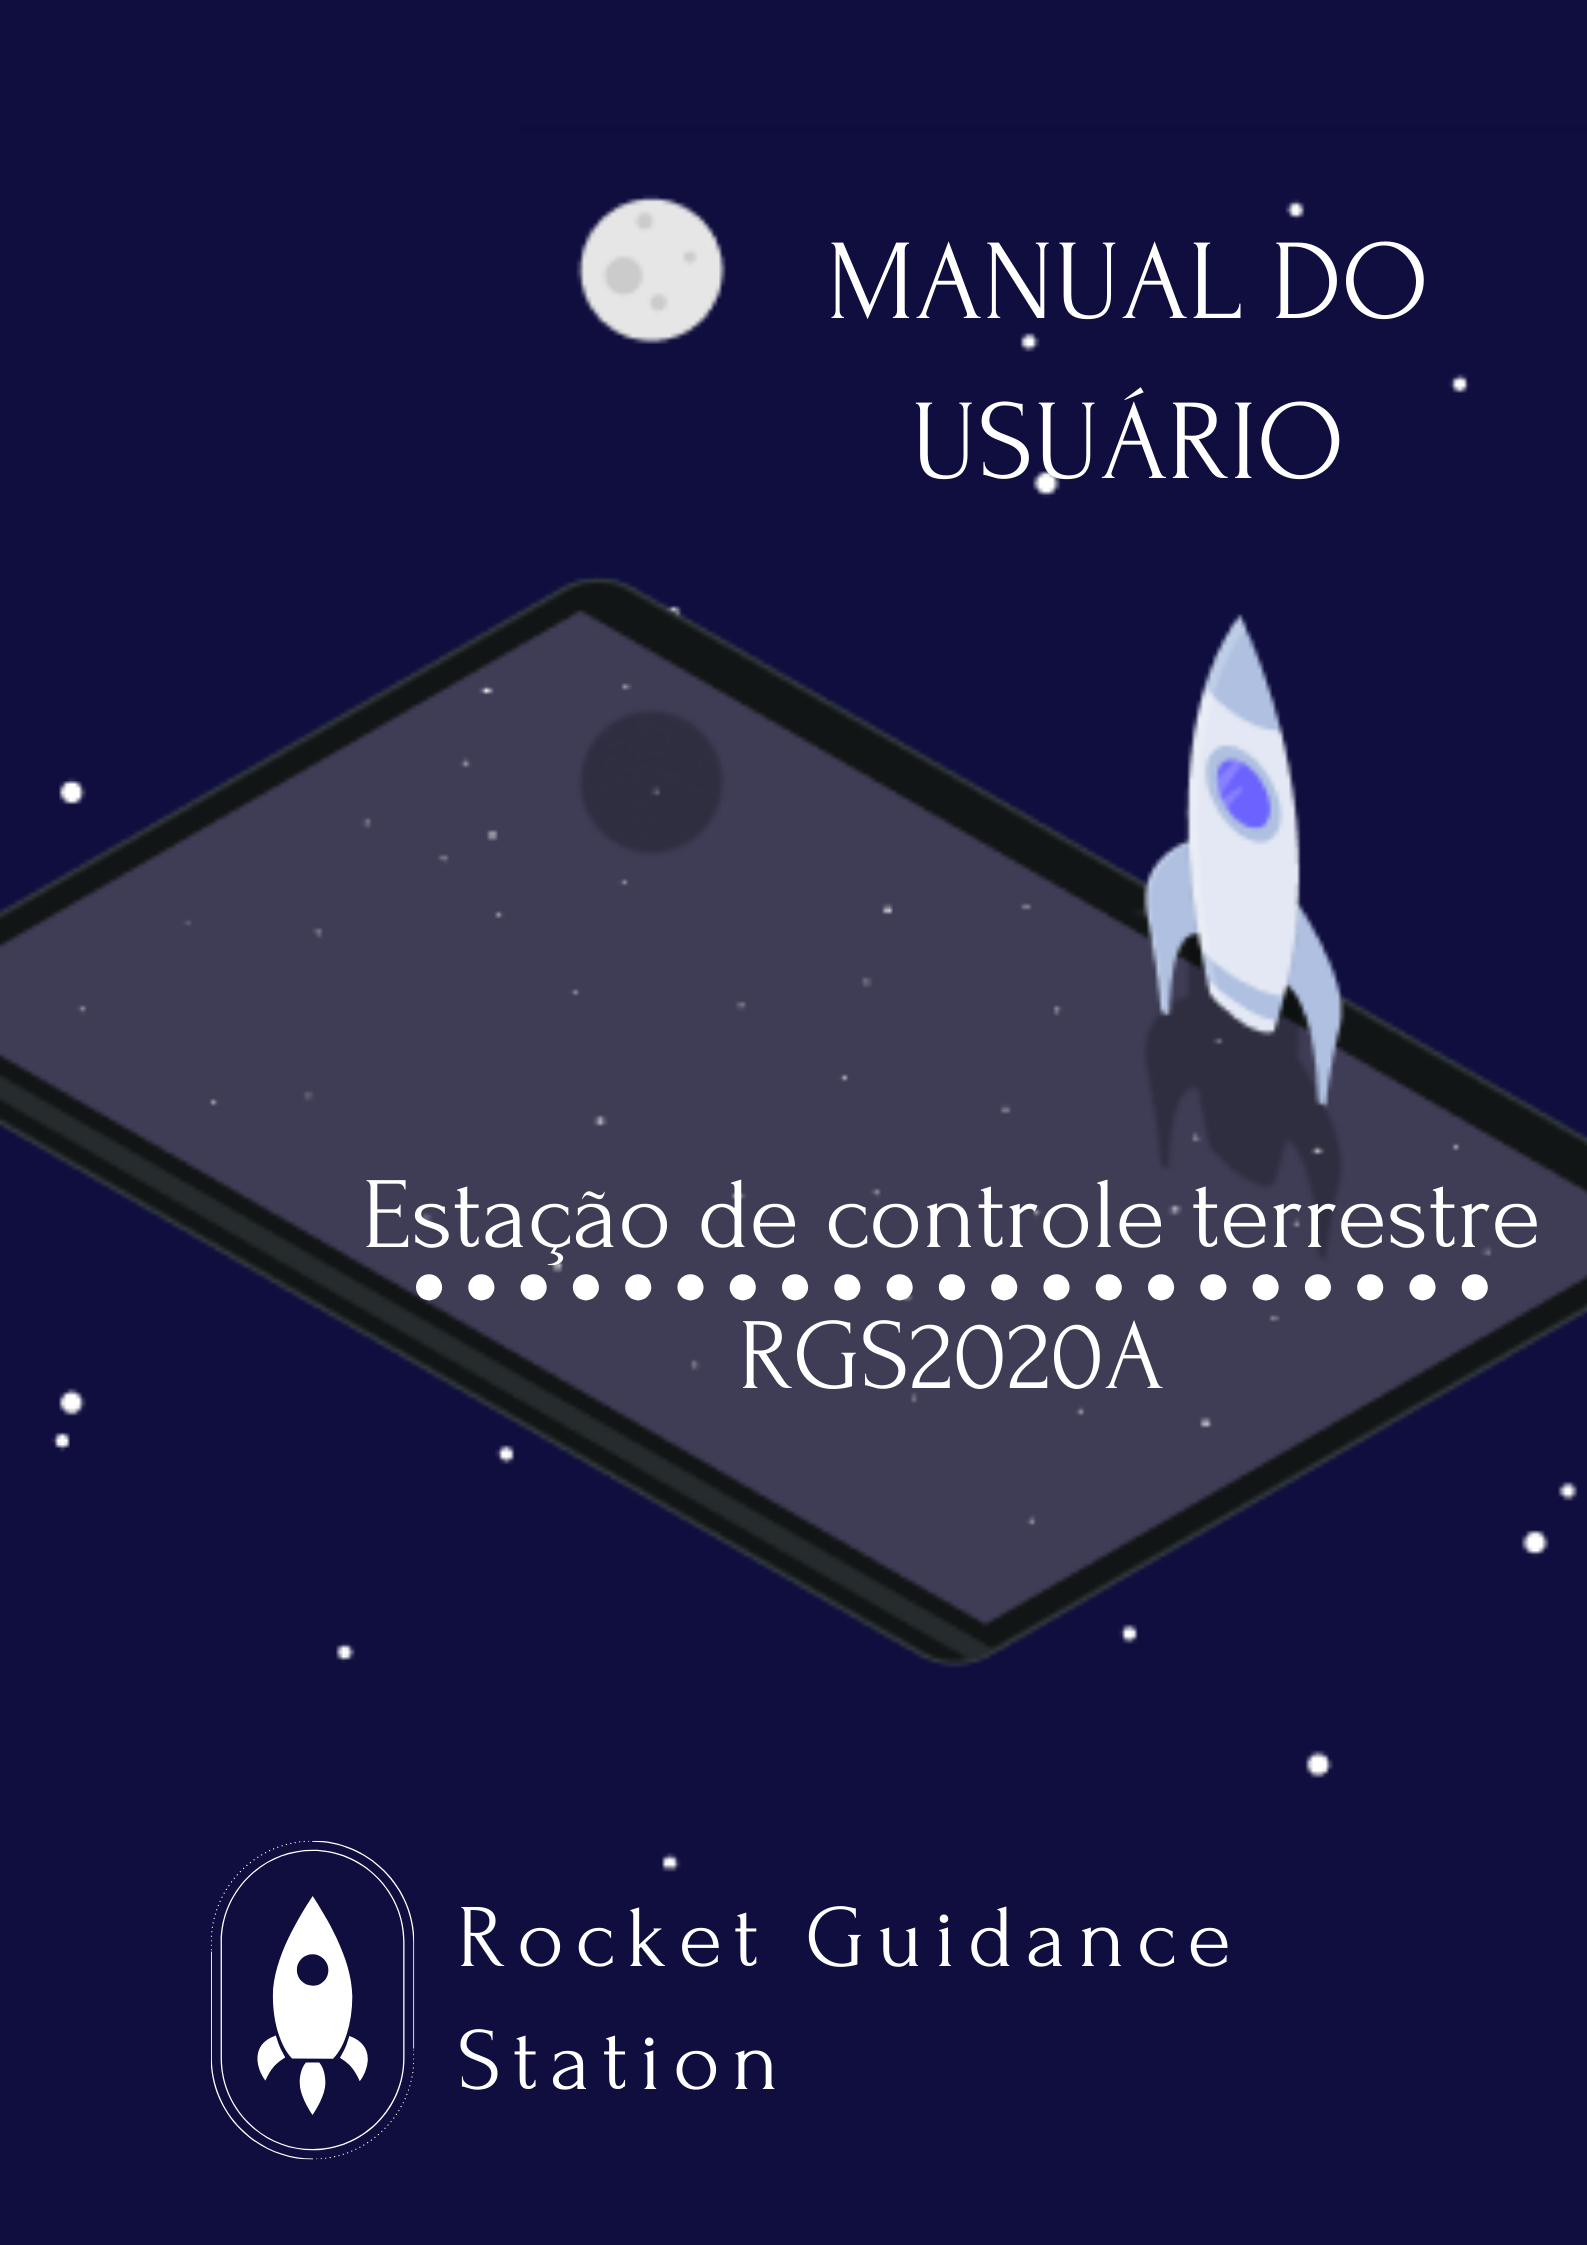
\includegraphics[width=\paperwidth\linewidth]{Figuras/capa.png}}} % Image background
\centering
\vspace*{11.3cm}
\par\normalfont\fontsize{35}{35}\sffamily\selectfont

\endgroup


%=========================================
\newpage{}
\thispagestyle {empty}

\vspace*{2cm}

\begin{center}

	\Large{\parbox{12cm}{
		\begin{raggedright}
		{\Large 
			Bem-vindo a família de produtos da Rocket Guidance Station.
 
			\vspace*{1cm}
			
			Antes de utilizar esse sistema leia e siga atentamente todas as informações do manual
			
			\vspace*{1cm}
			
			O RGS2020A é um sistema de apoio ao lançador de foguete experimental projetado para um lançamento eficiente e seguro do seu foguete. Para o melhor desempenho do mesmo leia todas as informações sobre segurança, instruções de instalação e operação, para evitar lesões ou danos ao usuário ou ao equipamento .
		}
	
		\vspace{.5cm}\hfill{RGS}
		\end{raggedright}
	}
}
\end{center}


\tableofcontents

\newpage
\chapter{Medidas de segurança}

\textbf{Leia essas medidas de segurança antes de utilizar o sistema. Elas contêm informações gerais de segurança. Siga as informações de aviso e de cuidado para evitar ferimentos a você mesmo ou a outras pessoas e para evitar danos ao produto.}

\section*{AVISO}

\begin{center}
 Avisos de segurança nível gravíssimo

\begin{figure}[H]
\centering

\includegraphics[scale = 0.2]{Figuras/aviso.png}
\end{figure}   
\end{center}


\begin{itemize}
    \item Não utilize cabos elétricos ou conectores danificados, nem tomadas desencaixadas ou danificadas, conexões pouco seguras podem causar choques elétricos ou incêndios.
    \item Não toque no sistema, nos cabos, nos conectores, no interruptor ou na tomada com as mãos molhadas ou outras partes do corpo molhadas.
    \item Não puxe os cabos além da extensão deles, isso pode causar choque elétrico ou incêndio.
    \item Não torça, nem danifique os cabos de eletricidade.
    \item Não faça a conexão direta dos pólos positivo e negativo do carregador ou da bateria.
    \item Não utilize o seu sistema ao ar livre durante tempestades.
    \item Não utilize baterias, carregadores, acessórios e equipamentos que não foram projetados para o sistema. Baterias, carregadores e cabos incompatíveis podem causar ferimentos em pessoas ou danos no aparelho.
    \item O uso de baterias ou carregadores genéricos poderá encurtar a vida útil do produto ou causar danos nele. Pode também causar incêndios ou fazer a bateria explodir.
    \item Não libere as válvulas sem garantir a despressurização do sistema.
    \item Não deixe cair nem cause impacto excessivo sobre as maletas e cases, isso pode danificar os equipamentos ou baterias, causar danos ou diminuir sua vida útil.
    \item Evite que os conectores e as extremidade do carregador entrem em contato com materiais condutivos como líquidos, poeira, pós de materiais metálicos e pontas de lápis. Não toque os conectores com ferramentas pontiagudas ou cause algum impacto neles. Você pode criar um curto-circuito ou corroer os terminais, o que pode resultar em explosão ou incêndio.
    \item Não deixe o sistema perto de crianças ou animais.
    \item Não manuseie uma bateria  danificada ou com vazamento
    \item Para o descarte seguro da bateria leia a seção descarte correto do sistema.
\end{itemize}

\section*{ATENÇÃO}

\begin{center}
    Avisos de segurança nível grave

\begin{figure}[H]
\centering

\includegraphics[scale = 0.1]{Figuras/atenção.png}
\end{figure}
\end{center}


\begin{itemize}

\item Atenção ao utilizar os dispositivos perto de outros aparelhos eletrônicos, pois os mesmos emitem um sinal de frequência que pode causar interferência.
\item Evite utilizar o produto perto de um marca-passo, porque poderá causar interferência. 
\item Se faz o uso de um equipamento médico, contate o fabricante do equipamento antes de usá-lo para determinar se o equipamento poderá ou não ser afetado pelas radiofrequências emitidas pela base.
\item Não acione o sistema de abastecimento perto do cilindro de propelente líquido.
\item Observe sempre os regulamentos, instruções e sinais de aviso nos ambientes de lançamento.
\item Se qualquer peça estiver quebrada, apresentar fumaça ou cheiro de queimado, pare de usá-lo imediatamente.
\item Mantenha as maletas e cases secas, umidade e líquidos podem danificar partes ou circuitos elétricos.
\item Não deixe nenhuma parte do produto cair, pois poderá danificar o sistema.
\item Se os pólos da bateria entrarem em contato com objetos metálicos, poderá ocorrer um incêndio.
\item Atenção a ambientes com altas temperaturas e campos magnéticos intensos. Poderá danificar a estrutura ou o sistema eletroeletrônico.
\item Não entre em contato com o sistema caso ele esteja superaquecido, poderá causar queimadoras na pele.
\item Certifique-se de que os equipamentos de instalação manual pelo usuário se encontram devidamente instalados antes do uso.
\item Utilize o sistema apenas para os fins aos quais se destina

\end{itemize}

\chapter{Memorial descritivo}

\section*{Conteúdo e acessórios}

\begin{table}[H]
\centering
\begin{tabular}{|l|l|l|}
\hline
Equipamento & Descrição  & Quantidade \\ \hline
Maleta de controle & Estrutura que comporta a interface de usuário & 1 \\ \hline
Maleta de suporte & Estrutura que armazena, transporta e alimenta os & \\ & equipamentos de abastecimento e ignição  & 1 \\ \hline
Adaptador dos & Sistema de acoplamento entre válvula e motor & \\ atuadores & & 2 \\ \hline
Mangueira & Mangueira de conexão entre adaptador e válvula anti-retorto & 1 \\ \hline
Válvula anti-retorno & Válvula que garante o transporto hidráulico em uma & \\ & única direção & 1 \\ \hline
Engate rápido & Conector com a parte interna do foguete & 1 \\ \hline
Carregador & Estrutura de carregamento das baterias & 1 \\ \hline
Módulo base de & Estrutura que controla os sensores da base de lançamento & \\ lançamento & e os atuadores do abastecimento & 1 \\ \hline
\end{tabular}
\end{table}

\section*{Maleta de controle}

\subsection*{Características}

\begin{figure}[H]
  \centering
  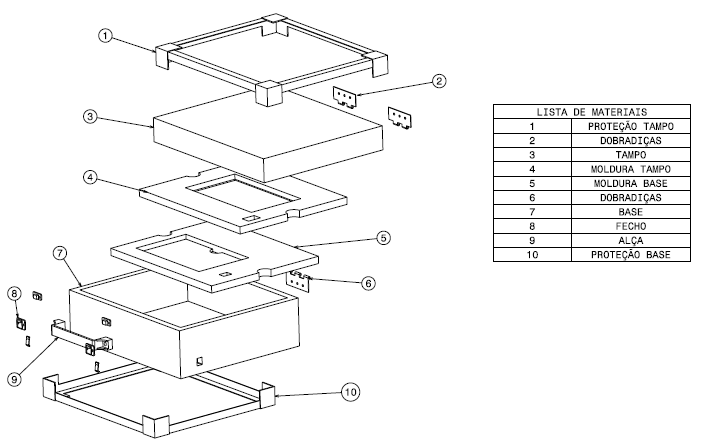
\includegraphics[scale=0.7]{Figuras/gcs_explode.png}
  \caption{Layout da Maleta de Controle - Estrutura}
  \label{fig:gcs_explode}
\end{figure}

\begin{figure}[H]
  \centering
  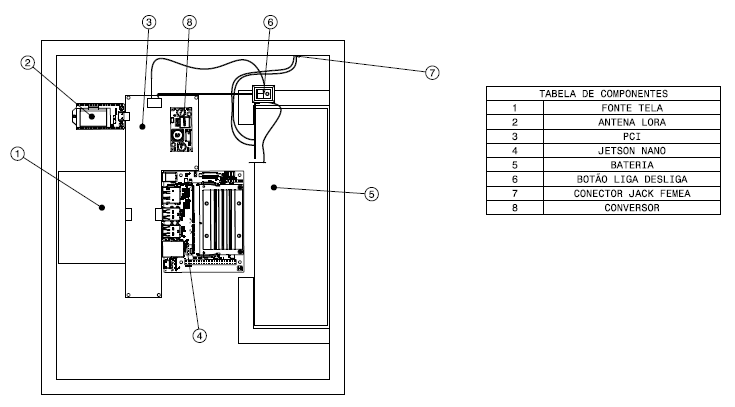
\includegraphics[scale=0.7]{Figuras/gcs_componentes.png}
  \caption{Layout da Maleta de Controle - Componentes}
  \label{fig:gcs_explode}
\end{figure}

\subsection*{Informações técnicas}

\begin{table}[H]
\centering
\begin{tabular}{|l|l|}
\hline
Modelo & RGS2020A-GCS \\ \hline
Tensão & 12V \\ \hline
%Frequência &  \\ \hline
Potência & 97 Wh \\ \hline
Dimensões & 352x300x152(mm) \\ \hline
Peso & 5 kg \\ \hline
Tamanho da tela & 9' \\ \hline
\end{tabular}
\end{table}

\subsection*{Instruções de uso}

\par Coloque a maleta sobre uma superfície nivelada, abra os fechos da maleta, indicados na imagem e depois aperte o botão de ligar/desligar para iniciar a missão.

\section*{Maleta de suporte}

\subsection*{Características}

\begin{figure}[H]
  \centering
  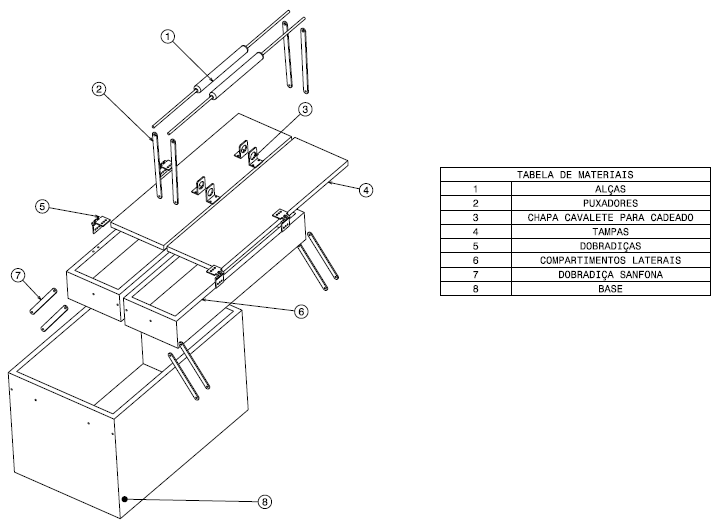
\includegraphics[scale=0.8]{Figuras/suporte_explode.png}
  \caption{Layout da Maleta de Suporte}
  \label{fig:suporte_explode}
\end{figure}

\subsection*{Informações técnicas}

\begin{table}[H]
\centering
\begin{tabular}{|l|l|}
\hline
Modelo & RGS2020A-Suporte \\ \hline
Tensão & 12V \\ \hline
%Frequência &  \\ \hline
Potência & 40 Wh \\ \hline
Dimensões & 520x330x568 (mm)\\ \hline
Peso & 10 kg \\ \hline
\end{tabular}
\end{table}

\subsection*{Instruções de uso}

\par Primeiro coloque as alças laterais para baixo, depois abra os cadeados e os retire dos cavaletes. Puxe as tampas para cima e abra os compartimentos superiores lateralmente. Retire os equipamentos removíveis da maleta, e monte-os de forma adequada. Por fim conecte os cabos de energia no local indicado para a alimentação do sistema dentro da maleta.

\section*{Carregador}

\subsection*{Características}

\begin{figure}[H]
  \centering
  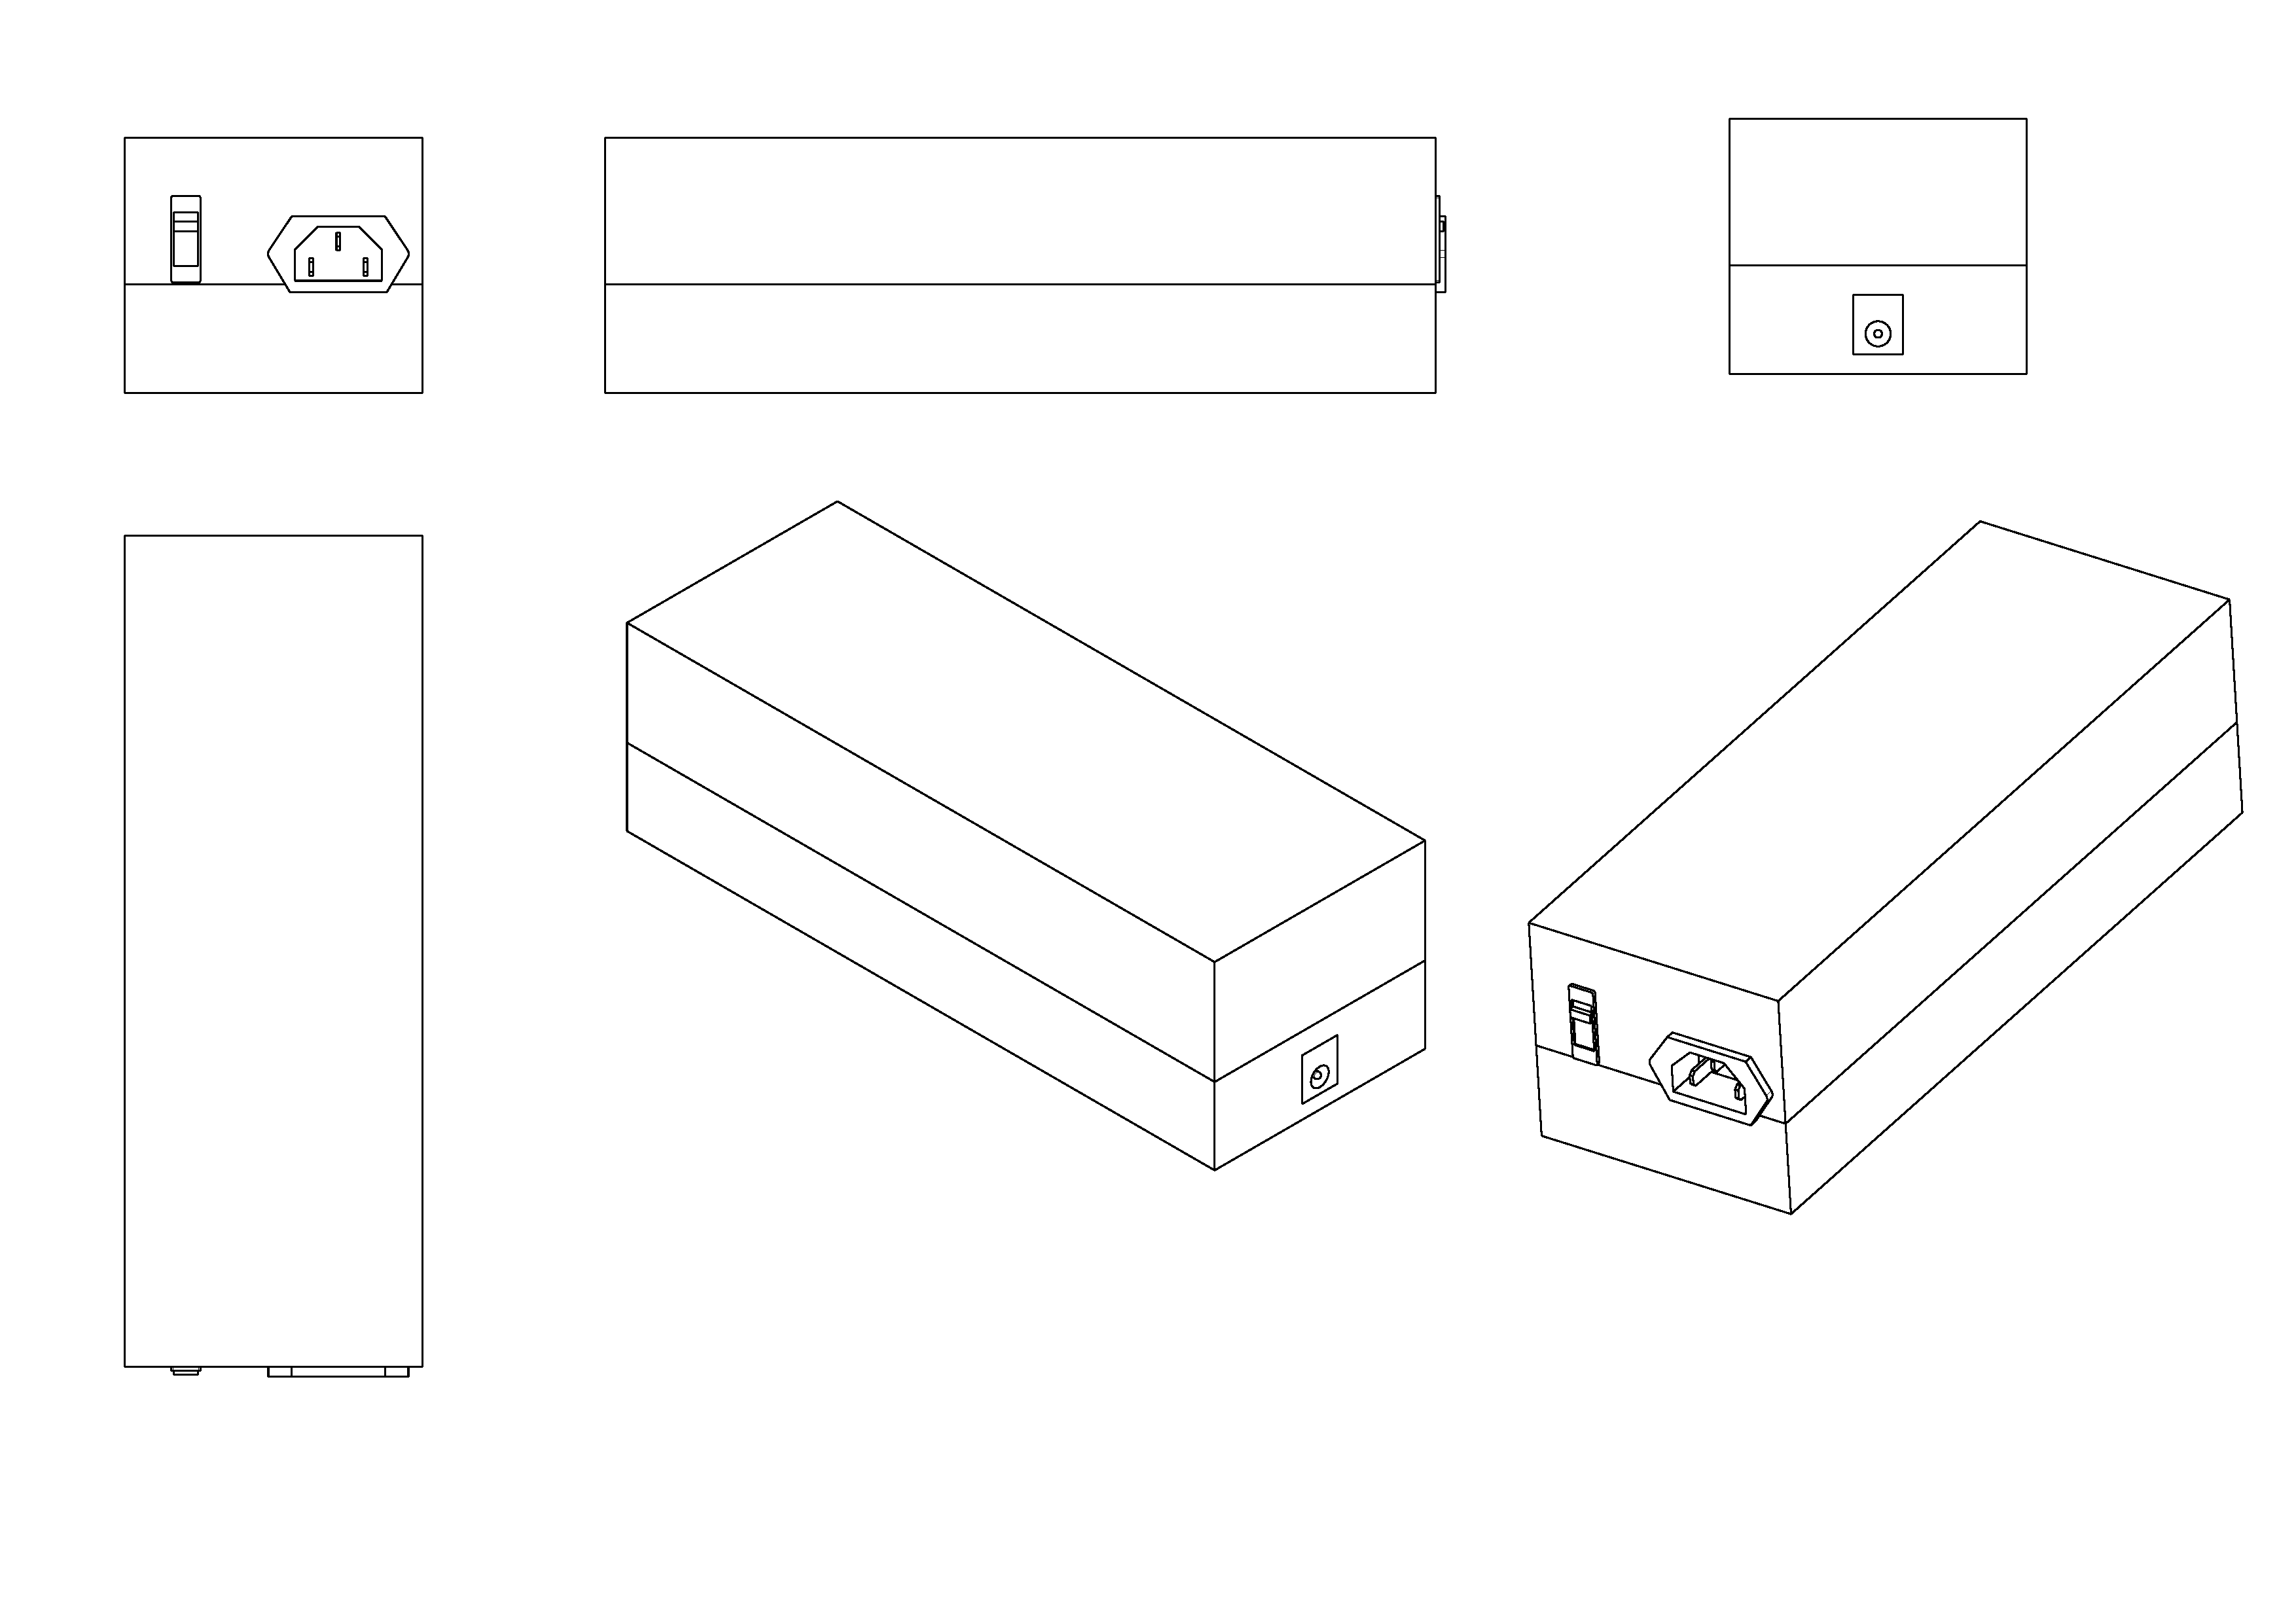
\includegraphics[scale=0.2]{Figuras/Vistas_carregador.pdf}
  \caption{Layout do Carregador}
  \label{fig:suporte_explode}
\end{figure}

\section*{Controlador da Base de lançamento}

\subsection*{Características}

\begin{figure}[H]
  \centering
  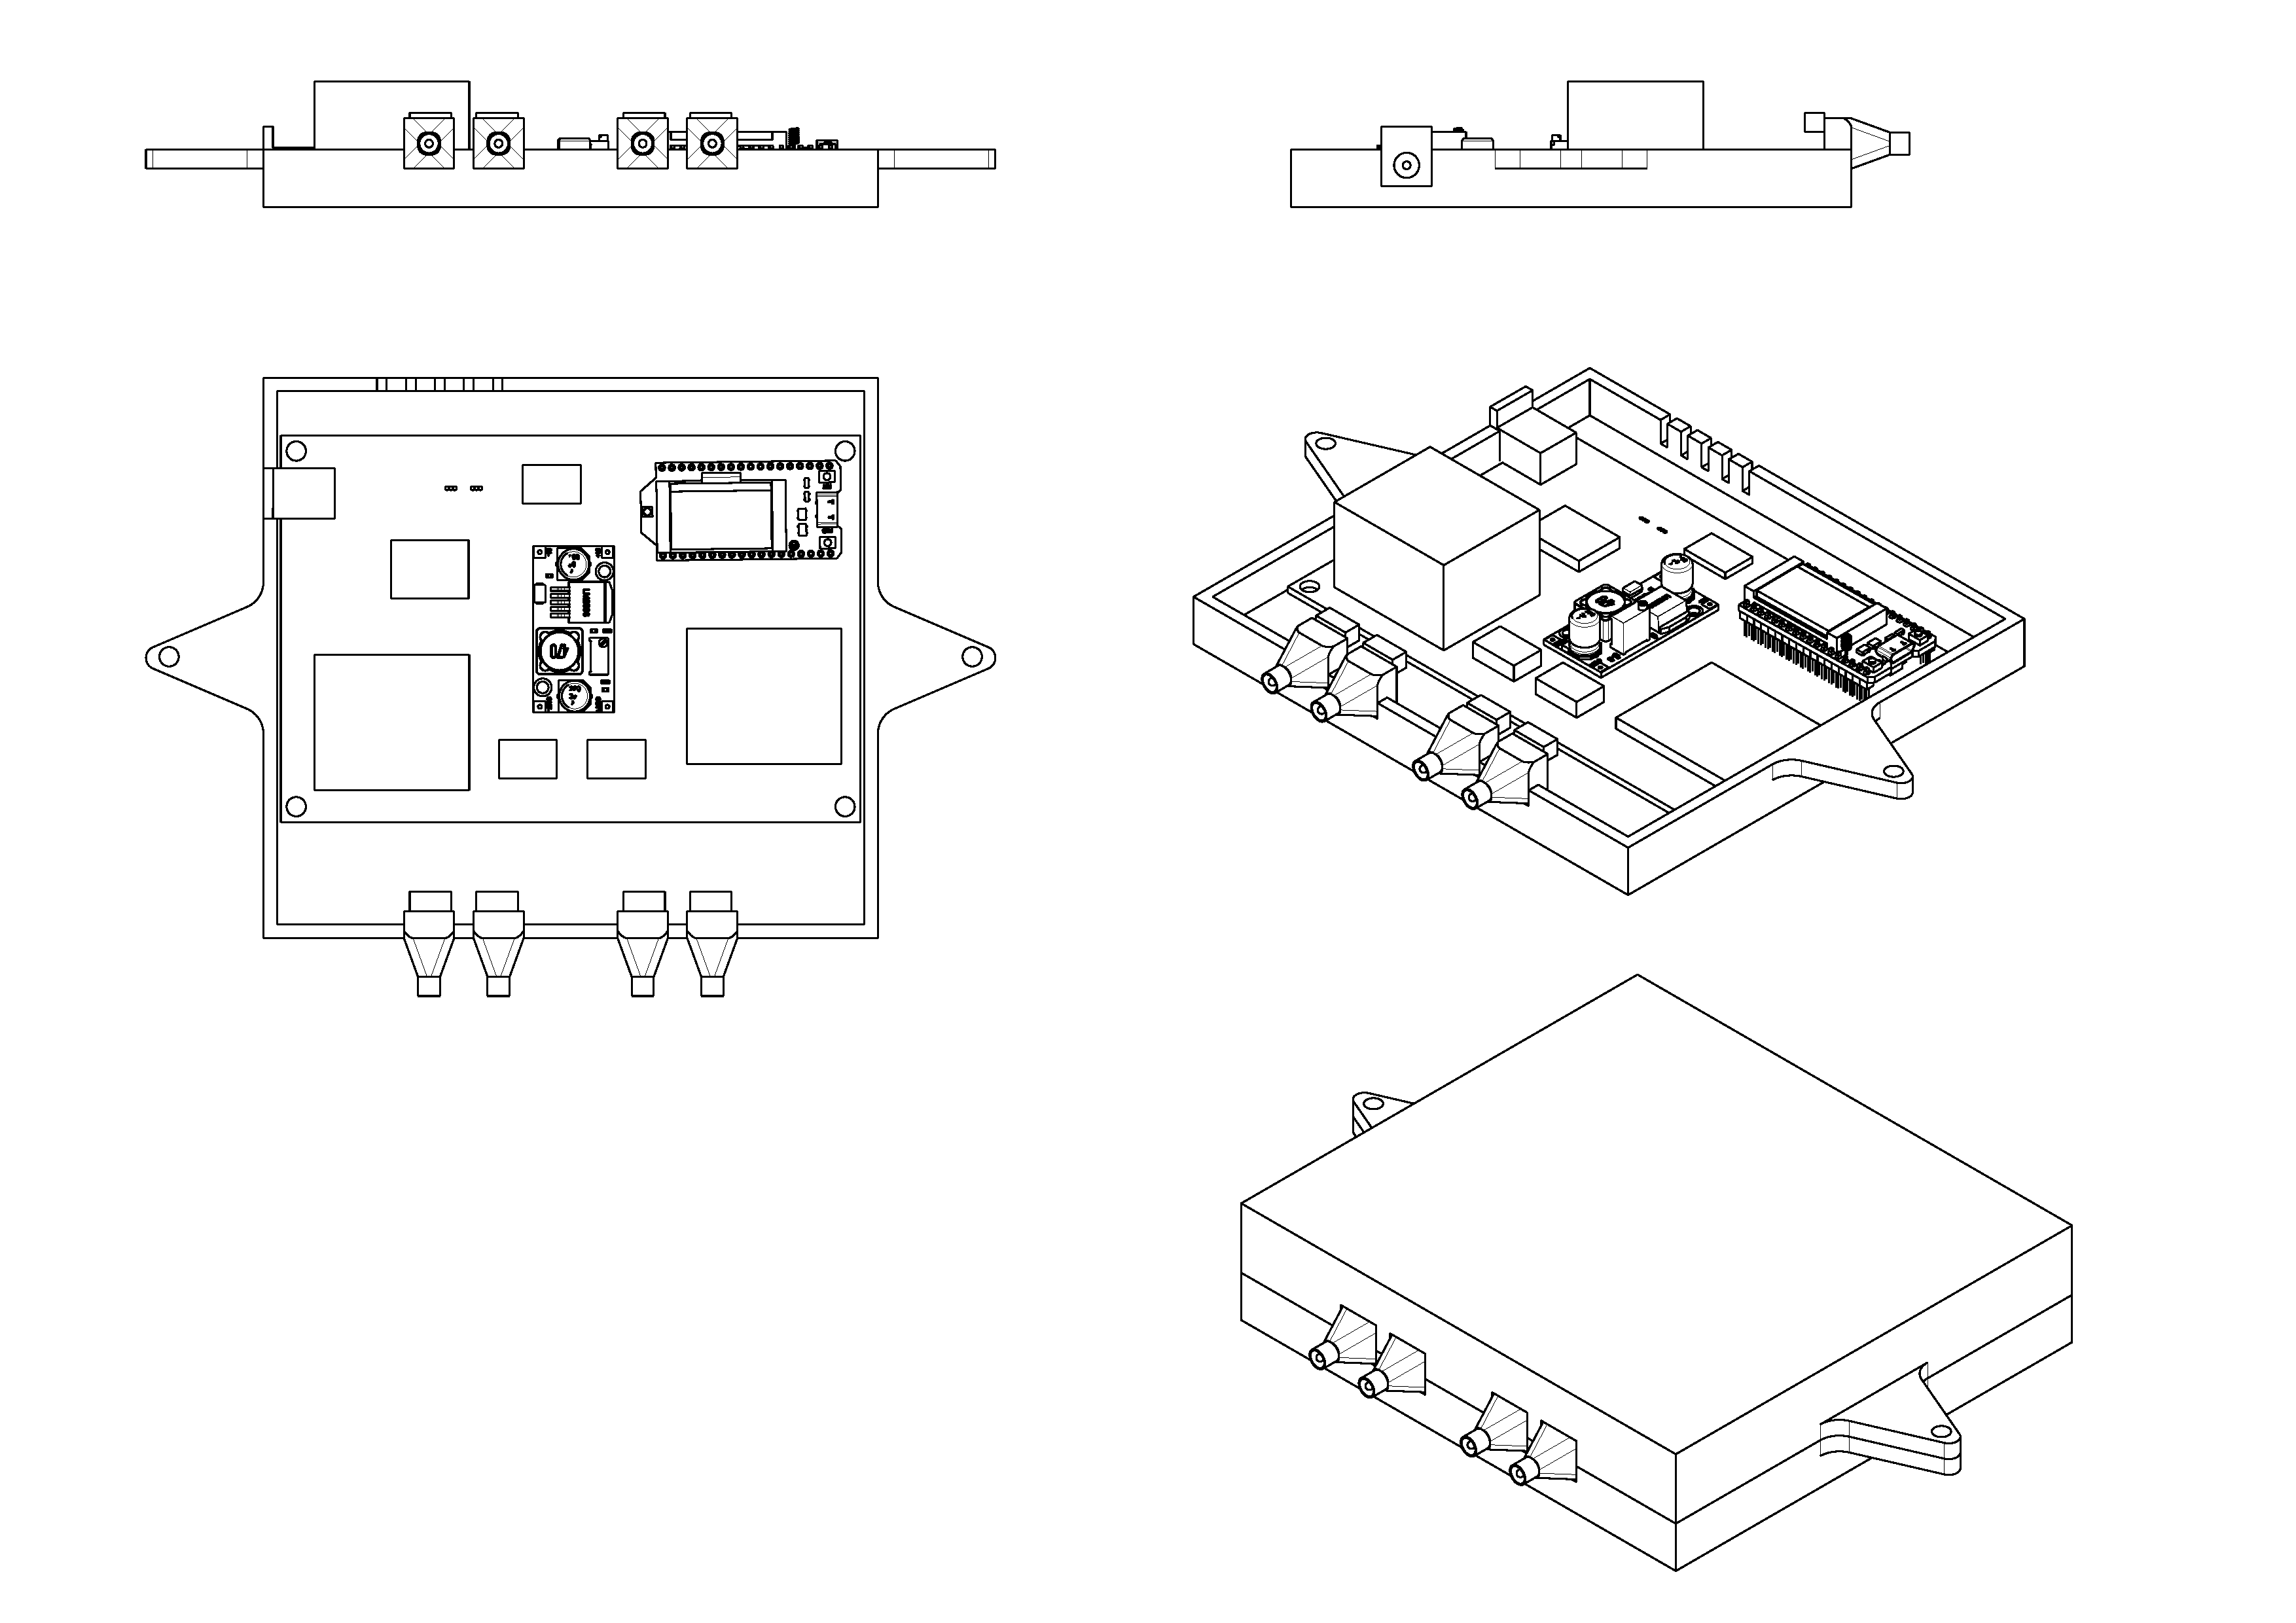
\includegraphics[scale=0.2]{Figuras/Vistas_caseelet.pdf}
  \caption{Layout do Controlador da Base de lançamento}
  \label{fig:suporte_explode}
\end{figure}

%\section*{Abastecimento}

%\subsection*{Características}

%\subsection*{Informações técnicas}

%\subsection*{Instruções de uso}

\section*{Dentro do Foguete}
\subsection*{Características}
\par Como o foguete é  uma caixa preta no projeto foi projetado um circuito completo e adaptável para ser adicionado dentro do foguete em uma PCI mostrada na figura \ref{fig:Dimensões da PCI do f} com as dimensões mostradas e com a opção de fixação dentro do foguete por parafusos de rosca m5.

\begin{figure}[H]
  \centering
  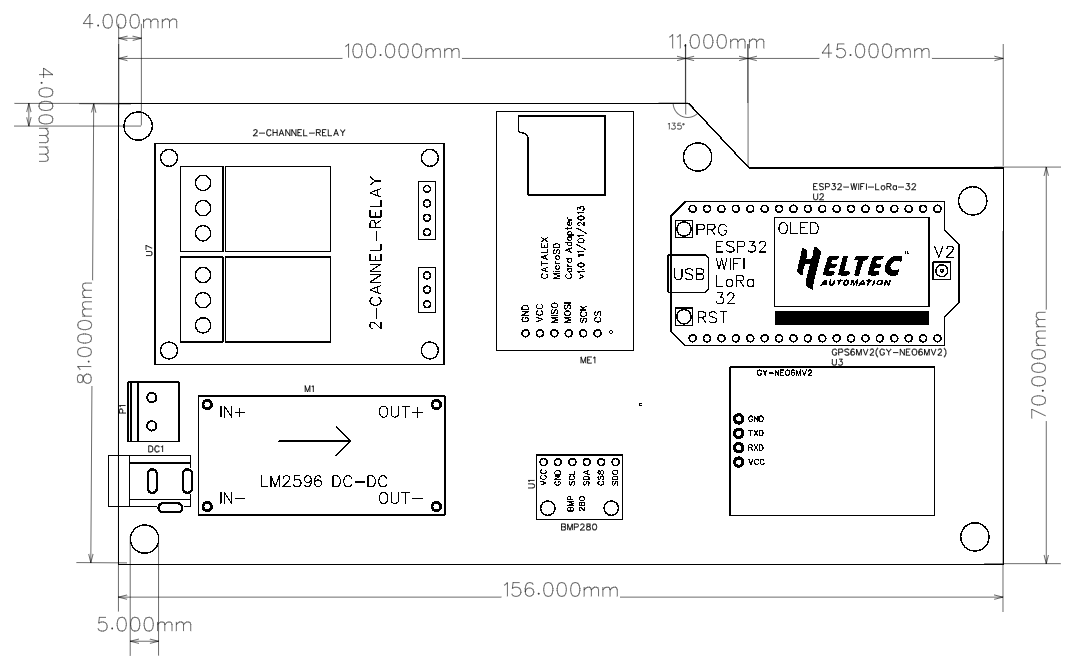
\includegraphics[scale=0.3]{Figuras/PCB_PCB_interna do foguete.png}
  \caption{Dimensões da PCI do foguete.}
  \label{fig:Dimensões da PCI do f}
\end{figure}

\subsection*{Informações técnicas}
\par A placa de circuito impresso do foguete foi projetada de forma a ser funcional e pequena para melhor acomodação dentro do foguete, há cinco furos para a fixação da mesma no foguete todas com rosca M5 possui demissões de 156.0 x 81.0 mm espessura de 1.6mm e espessura de cobre de 1$oz$.

\subsection*{Instruções de uso}

\par Para a utilização do circuito do foguete inicialmente é necessário a gravação da ESP 32 LoRa com auxílio de um cabo Micro-USB e um computador pessoal.Para isso é necessário ter a IDE do Arduíno instalado no computador pessoal, pode ser obtida através do link : https://www.arduino.cc/en/software e siga os passos abaixo:
\begin{itemize}
    \item Apos entrar no site clique no local indicado na figura \ref{fig:Download ide} e faça o download para a versão do seu sistema operacional;
    \begin{figure}[H]
  \centering
  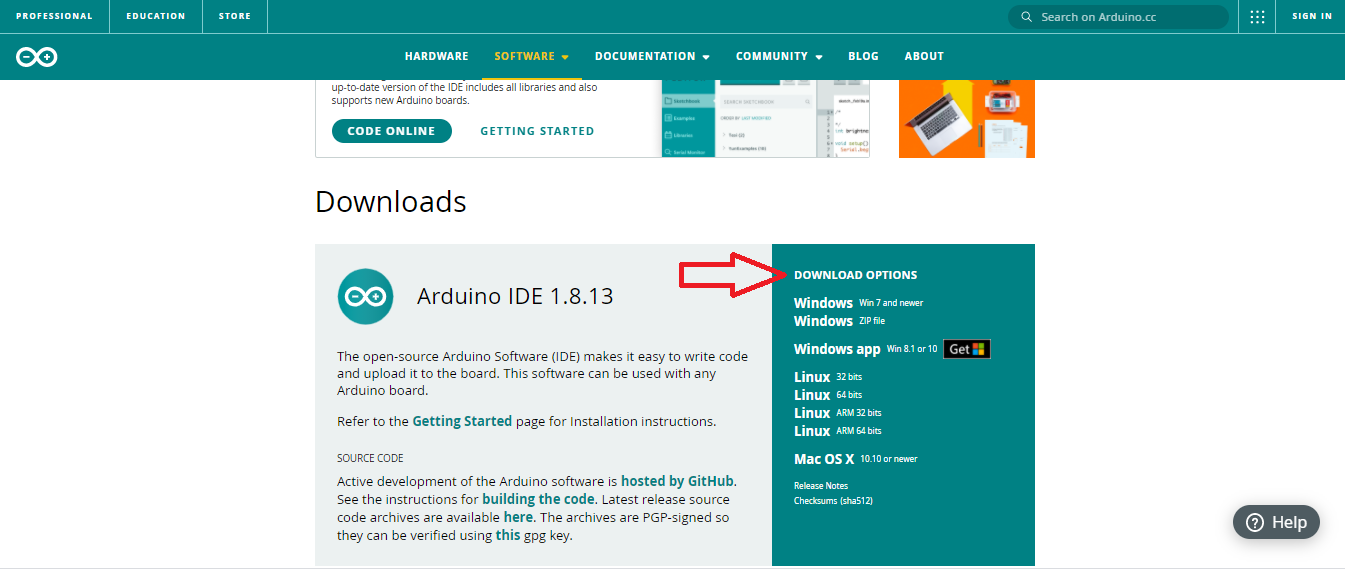
\includegraphics[scale=0.4]{Figuras/passo1.png}
  \caption{Passo 1 - Download IDE}
  \label{fig:Download ide}
\end{figure}
\item Apos o download basta instalar o programa.
\item Clique na aba Arquivos e em seguida em preferências;
   \begin{figure}[H]
  \centering
  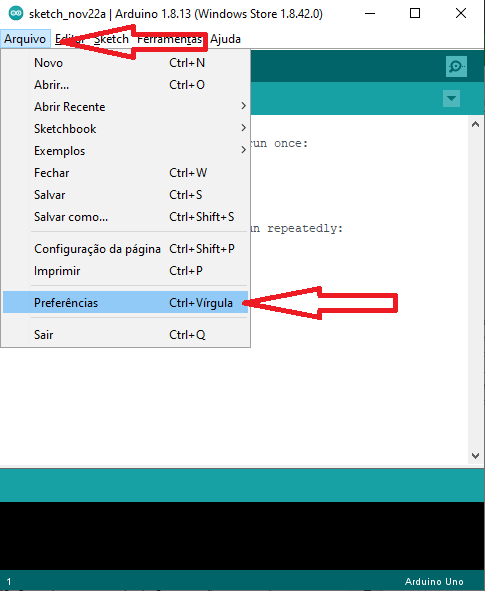
\includegraphics[scale=0.4]{Figuras/passo2.png}
  \caption{Passo 2}
  \label{fig:Download ide}
\end{figure}

\item Adicione a URL para instalação do pacote da ESP32 \\https://dl.espressif.com/dl/package_esp32_index.json

   \begin{figure}[H]
  \centering
  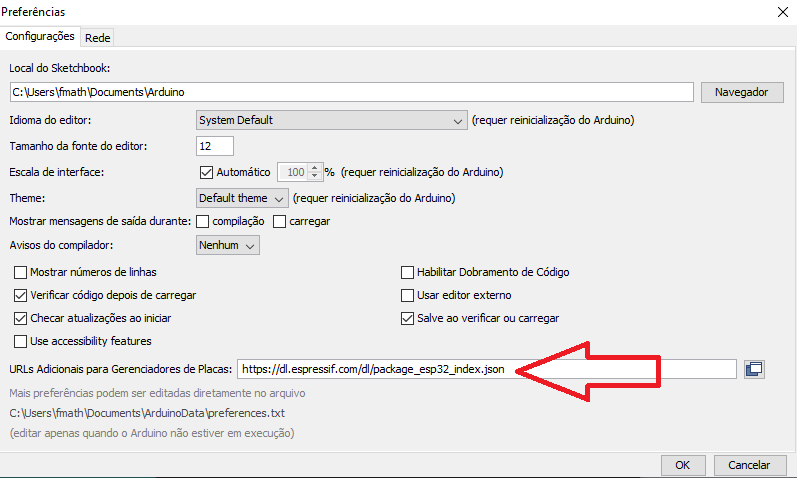
\includegraphics[scale=0.4]{Figuras/passo3.png}
  \caption{Passo 3}
  \label{fig:Download ide}
\end{figure}

\item Vá no ícone \textbf{ Ferramentas/Placa:"Arduino Uno"/gerenciador de Placas...}

   \begin{figure}[H]
  \centering
  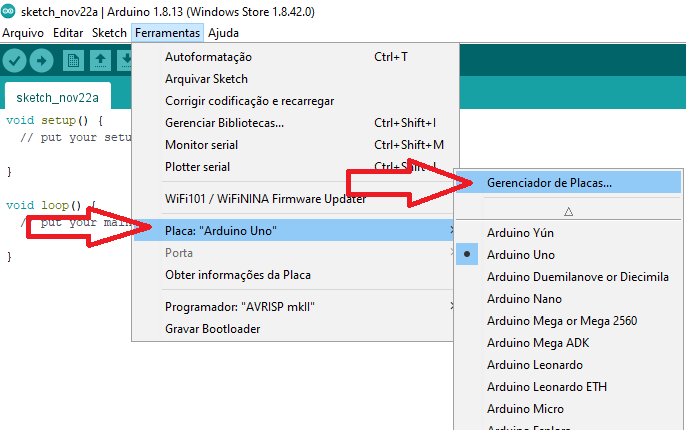
\includegraphics[scale=0.4]{Figuras/passo4.png}
  \caption{Passo 4}
  \label{fig:Download ide}
\end{figure}
\item Pesquise por ESP32 na aba de pesquisa e clique em instalar nos arquivos da ESP32.
   \begin{figure}[H]
  \centering
  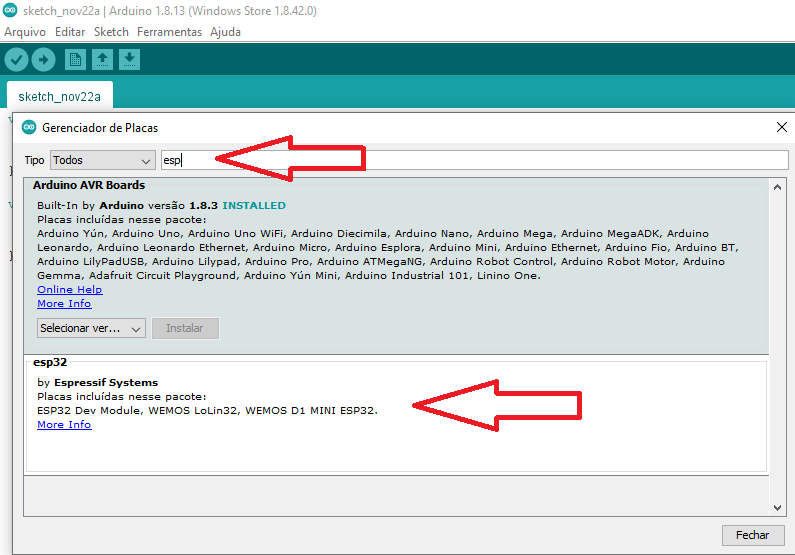
\includegraphics[scale=0.4]{Figuras/passo5.png}
  \caption{Passo 5}
  \label{fig:Download ide}
\end{figure}
\item Vá no ícone\textbf{ Sketch/Inclui Biblioteca/Gerenciador de Bibliotecas...}
   \begin{figure}[H]
  \centering
  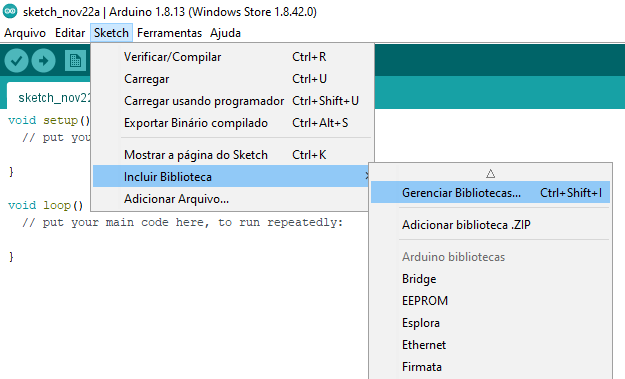
\includegraphics[scale=0.4]{Figuras/passo6.png}
  \caption{Passo 6}
  \label{fig:Download ide}
\end{figure}
\item Pesquise por HELTEC na aba de pesquisa e clique em instalar .
   \begin{figure}[H]
  \centering
  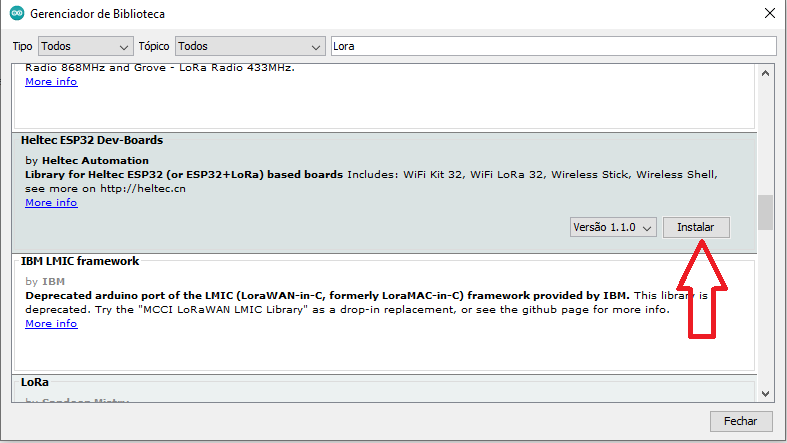
\includegraphics[scale=0.4]{Figuras/passo7.png}
  \caption{Passo 7}
  \label{fig:Download ide}
\end{figure}
\item Pesquise por LoRa na aba de pesquisa e clique em instalar .
   \begin{figure}[H]
  \centering
  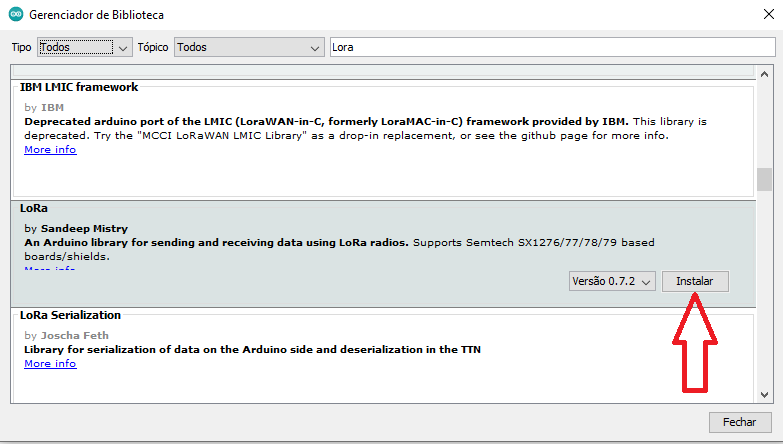
\includegraphics[scale=0.4]{Figuras/passo8.png}
  \caption{Passo 8}
  \label{fig:Download ide}
\end{figure}

\item Apos a instalação do programa e bibliotecas necessárias basta utilizar um cabo Micro-USB\ref{fig:Cabo MicroUSB}  conectado a ESP32 LoRa da Heltech e a um computador pessoal que esteja com as etapas acima feitas e instalar o código disponibilizado para o funcionamento do hardware em questão.
   \begin{figure}[H]
  \centering
  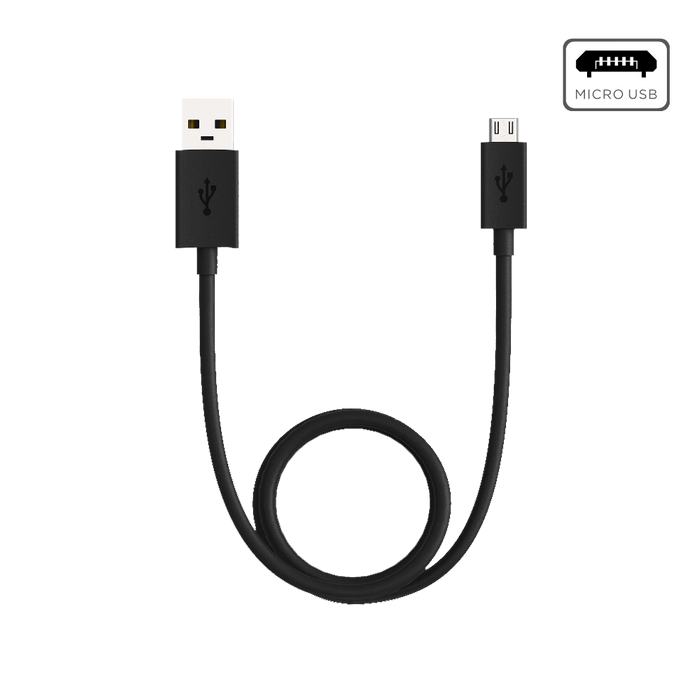
\includegraphics[scale=0.4]{Figuras/25.carregador-image-usb.png}
  \caption{Cabo MicroUSB}
  \label{fig:Cabo MicroUSB}
\end{figure}

    
\end{itemize}
% 
\chapter{Calibração}

\section*{Célula de carga}
\begin{center}
    \begin{figure}[H]
    \centering
		
\includegraphics[scale=1.6]{Figuras/bateria/iconeimportante.png}
	    \label{iconeimportante}
    \end{figure} 
  
    	Informação importante sobre \textbf{CALIBRAÇÃO}
 \end{center}  

\par Dentre os sensores utilizados na base de lançamento e no foguete, apenas as células de cargas da balança são transdutores necessários de calibração, os demais sensores já possuem calibração de fábrica, onde geralmente seus coeficientes de calibragem ficam armazenados em ROM.

\par Para calibrar a balança, após a montagem com as duas células de carga 50 Kg e o módulo conversor HX711, será executado uma rotina de ajuste do sistema de medição em código C no microcontrolador ESP32 LoRa. De acordo com o Vocabulário Internacional de Metrologia Legal (VIML) o ajuste de um sistema de medição é conjunto de operações efetuadas num sistema de medição, de modo que ele forneça indicações prescritas correspondentes a determinados valores de uma grandeza a ser medida. 

\par Através do programa executado deve ser encontrado um valor aferido  denominado como Fator de Ajuste para  ser inserido no programa de medição da Balança com o conversor, e assim a calibração seja realizada.

\par O programa de ajuste fará uso da biblioteca \href{https://github.com/bogde/HX711}{HX711.h}, onde um objeto de peso conhecido deve ser lido pela balança, e a média dos valores retornados deve ser dividido pelo valor do peso real do objeto em KG, obtendo o fator de ajuste, que deve ser inserido como parâmetro da função “scale.set\textunderscore scale()” importada da biblioteca mencionada. Com esse fator de ajuste setado, obtém-se a calibração da balança, medindo então o do peso real do objeto.

\par A figura \ref{fig:Calibracao_balanca} apresenta o fluxograma do algoritmo de ajuste e calibração dos sensores da balança.

\begin{figure}[H]
  \centering
  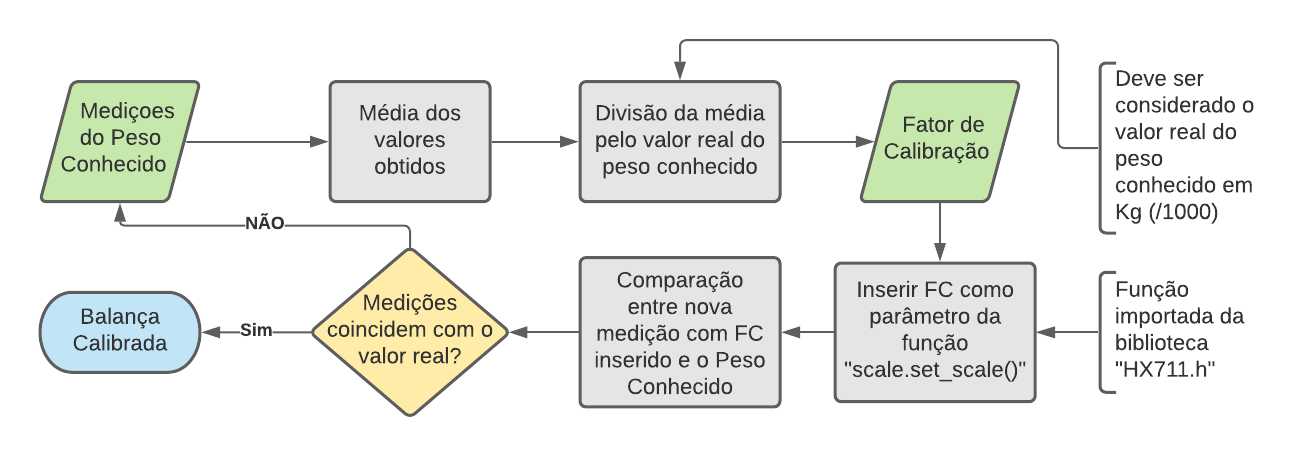
\includegraphics[width=\textwidth]{Figuras/Algoritmo de Calibração da Balança.png}
  \caption{Diagrama do algoritmo de calibração da balança } 
  {\footnotesize Fonte : Autor } 
  \label{fig:Calibracao_balanca}
\end{figure}

\chapter{Bateria}

\section*{Informações de segurança}

Leia toda a informação de segurança descrita nesta seção antes de instalar e de operar o equipamento. Não negligencie nenhuma instrução.

Para manipular e operar os sistemas de baterias:

\begin{itemize}

    \item Você deve ter qualificação para trabalhos com eletricidade;
    \item Remover todo e qualquer adereço metálico como joias, relógios, pulseiras, canetas e
barras metálicas antes de começar a manusear a bateria;
    \item Usar somente ferramentas eletricamente isoladas.

\end{itemize}

\subsection*{Simbologia de segurança e recomendações}


\begin{center}
    \begin{figure}[H]
    \centering
		
\includegraphics[scale=1.6]{Figuras/bateria/iconeimportante.png}
	    \label{iconeimportante}
    \end{figure} 
  
    	Informação importante sobre \textbf{SEGURANÇA}
 \end{center}   	
 
 \begin{center}
  
    \begin{figure}[H]
       \centering
	\label{iconefogo}					
\includegraphics[keepaspectratio=true,scale=0.13]{Figuras/bateria/iconefogo.jpg}
        \label{iconefogo}
	\end{figure} 
		\textbf{NÃO} atirar a bateria ao fogo
\end{center}

\begin{center}
    \begin{figure}[H]
\centering
	\label{iconereciclar}					
\includegraphics[keepaspectratio=true,scale=0.13]{Figuras/bateria/iconereciclar.png}
        \label{iconereciclar}
	
	\end{figure} 
	\textbf{RECICLAR} ou descartar corretamente à bateria
 \end{center}   
 
 \begin{center}

  \begin{figure}[H]
  \centering
	\label{iconelixo}					
\includegraphics[keepaspectratio=true,scale=0.7]{Figuras/bateria/iconelixo.jpg}
        \label{iconelixo}
	
	\end{figure} 
      \textbf{NÃO} descartar a bateria em lixo comum.
 \end{center}  
\subsection*{Cuidados}
    
    \begin{figure}[H]
    \centering
	\label{iconeimportante}
		
\includegraphics[keepaspectratio=true,scale=1.4]{Figuras/bateria/iconeimportante.png}
	\label{iconeimportante}
	\end{figure} 
    
    \begin{enumerate}
    \item \textbf{NÃO} colocar a bateria na água. Armazenar a bateria em local fresco e seco, sem incidência direta do sol.
	\item \textbf{NÃO }aquecer ou jogar a bateria no fogo. Risco de explosão e/ou incêndio. 
\item Quando recarregar a bateria, utilizar equipamento especialmente projetado para isso e seguir os corretos procedimentos e parâmetros de uso. \textbf{NÃO }utilizar carregadores inadequados ou fora da especificação. \textbf{NÃO} realizar adaptações.
\item  \textbf{NÃO} reverter a polaridade da bateria. \textbf{NÃO} conectar a bateria diretamente na rede AC e evitar o curto-circuito entre os terminais.
\item  \textbf{NÃO} utilizar a bateria caso ela se torne quente, abaulada, deformada ou que apresente vazamentos.
\item \textbf{NÃO} perfurar a bateria. \textbf{NÃO } jogar, amassar ou causar impacto físico à bateria.
\item \textbf{NÃO} abrir ou tentar reparar a bateria em caso de defeito pois, além de perigoso, a garantia é invalidada caso ela tenha sido aberta para reparo por pessoal não autorizado pelo fornecedor.
\item \textbf{NÃO} descartar a bateria no lixo comum, procurar pontos de recolhimento para a correta destinação ou reciclagem.
    \end{enumerate}

    \subsection*{Precauções}
\begin{figure}[H]
\centering
	\label{iconeimportante}
		
\includegraphics[keepaspectratio=true,scale=1.6]{Figuras/bateria/iconeimportante.png}
	\label{iconeimportante}
	\end{figure} 
    
\begin{enumerate}
\item Caso a bateria esteja aquecida, abaulada, com odor ou aspecto anormal, entrar imediatamente em contato com o suporte e não usar a bateria.
\item  Caso precise armazenar a bateria por longos períodos, realizar uma carga e descarga com a bateria a cada 3 meses. Para assegurar o melhor desempenho e o melhor estado de carga, manter a bateria armazenada com carga entre 50\% e 60\%.
\item Utilizar a bateria apenas na faixa de temperatura adequada, entre -20ºC e 60ºC.
\item Antes da primeira utilização é recomendado recarregar a bateria.
\end{enumerate}
\newpage   

\section*{Troca das baterias}
\begin{figure}[H]
\centering
	\label{iconeimportante}
		
\includegraphics[keepaspectratio=true,scale=1.7]{Figuras/bateria/iconeimportante.png}
		
\includegraphics[keepaspectratio=true,scale=0.5]{Figuras/bateria/iconelixo.jpg}
	\label{iconeimportante}
	\end{figure} 
As baterias têm vida útil variável, e após determinado número de ciclos, de carga e descarga, perdem a capacidade de carga e devem ser substituídas.

Estima-se que o número de ciclos antes que ocorra essa perca na capacidade de carga seja superior a 4000. Porém, esse número pode variar de acordo com as condições de operação, armazenamento e recarga das baterias. 

Portanto, deve-se observar a situação de capacidade de carga das baterias periodicamente para se atentar a necessidade de trocas. A cada três meses recomenda-se ligar o sistema completo para testar por quanto tempo as baterias são capazes de manter todos os componentes alimentados. Dessa forma é possível observar a redução da capacidade das baterias com o passar do tempo e realizar a troca quando essa capacidade estiver muito próxima do necessário para os lançamentos remotos.

Para realizar a troca garanta que o dispositivo esteja desconectado da rede elétrica, então obedecendo todas as normas de segurança já estabelecidas nesse manual, retire a estrutura que protege a bateria usando chave de fenda, após isso desconecte todos os fios que estão presos a bateria com muito cuidado, no caso da bateria da maleta apenas desconecte o conector dock acoplado ao polos da bateria, depois troque pela nova bateria que deve ser do mesmo tipo (tamanho, tensão e capacidade) que a antiga. 

Depois de colocar a bateria nova no lugar repita as conexões que estavam na bateria anterior com cuidado e observando onde é o polo positivo (conexões com os fios de cor vermelha) e o polo negativo (conexões com os fios de cor preta) da bateria, no caso da bateria da maleta apenas conecte novamente o conector dock nos polos. Depois de conectado volte a estrutura para o lugar e fixe com os parafusos.

\section*{Carregamento das baterias}

\subsection*{Tensão de alimentação do carregador}
  
Conferir a tensão de alimentação selecionada, 110V ou 220V, antes de cada uso. Selecionar a tensão de acordo com o rede elétrica do local de uso por meio da chave seletora de tensão, localizada na estrutura do carregador.

\subsection*{Carregando as baterias}

As baterias devem ser recarregadas após cada uso. 

Ao retornar com o sistema para um local com acesso à rede elétrica, conectar os cabos à caixa do carregador, selecionar a tensão de alimentação adequada no carregador e conectar os cabos à tomada e ao plugue P4 indicado para carregamento da bateria na estrutura do sistema. 

A conexão à rede deve ser contínua por 3 horas ininterruptas, após esse período mínimo a bateria estará carregada, não há problema em deixar a bateria conectada à rede por períodos mais longos, pois o circuito de carregamento faz o controle da tensão para manter a carga. 

Após carregar o primeiro sistema, maleta ou base de lançamento, repetir o procedimento para o segundo sistema.

\chapter{Interface de Usuário}

Para facilitar a utilização do sistema,  colocamos à disposição a indicação de uso das principais features disponíveis para uso. Em prol do melhor entendimento  a ordem de apresentação das features será a mesma ordem de workflow básico do software.

Após a inicialização do software, a tela de criação do foguete será apresentada ao usuário, é a tela de criação de foguete. Nessa tela deve-se preencher os dados corretamente , selecionar as opções desejadas para o foguete  , clicar no botão 'criar foguete' e aguardar a confirmação do sistema , como pode ser observado na Figura \ref{teladecriacao}. 
\begin{center}

\begin{figure}[H]
\centering				            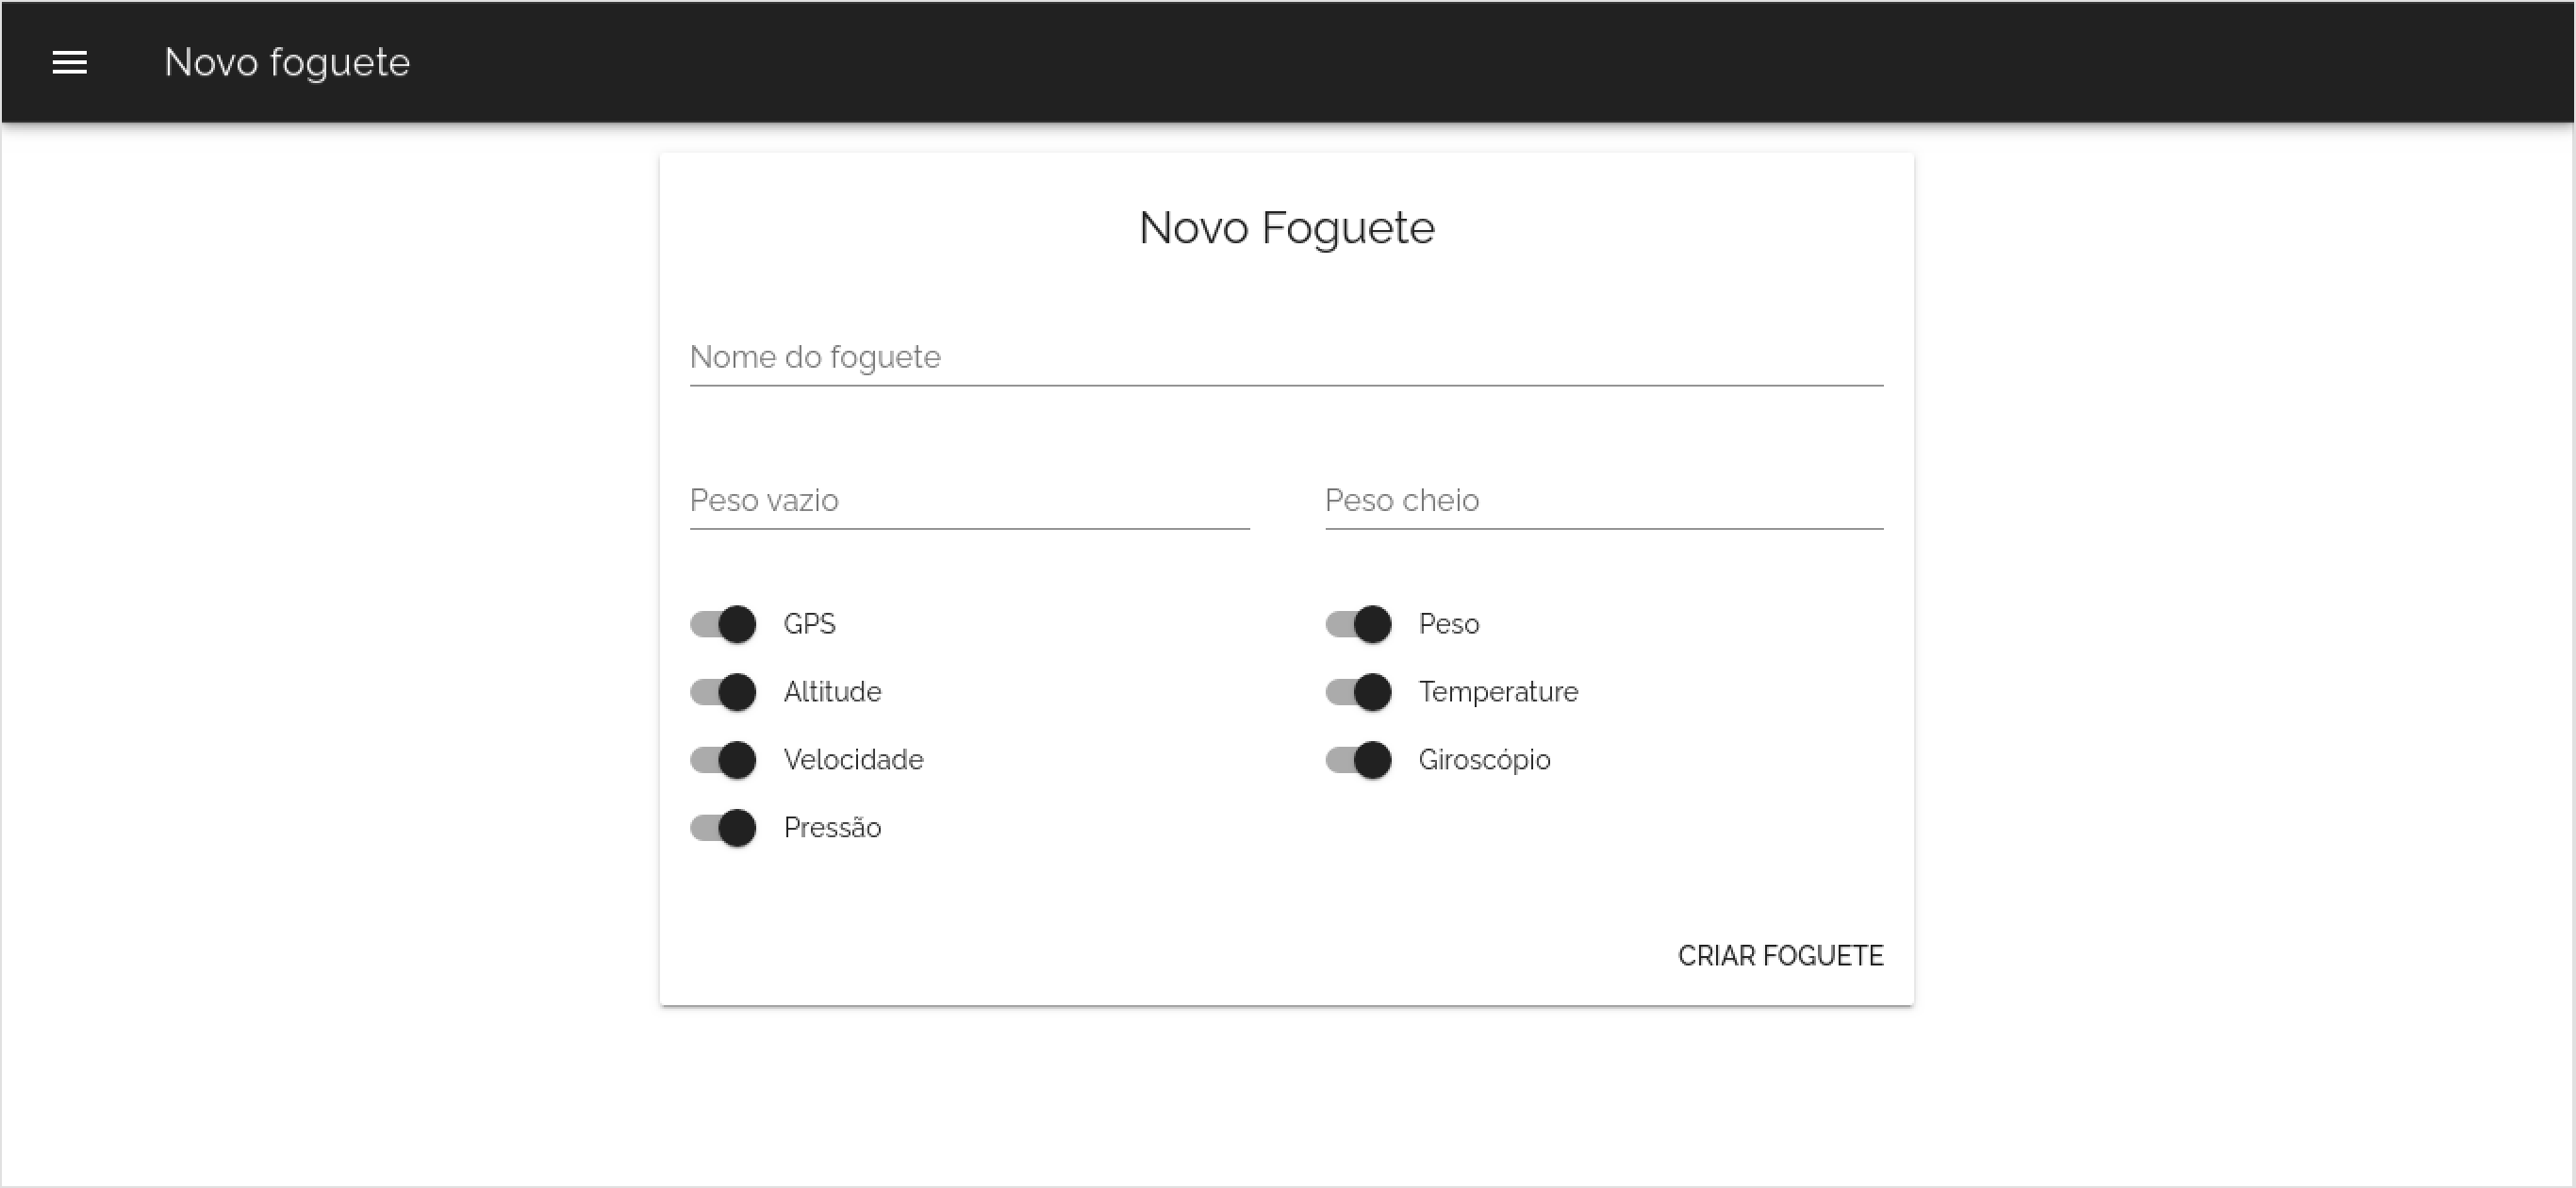
\includegraphics[width=\textwidth]{Figuras/telas/1.png}
        \label{teladecriacao}
	\caption{Tela de criação de novo foguete}
\end{figure} 
\end{center}

Na Figura \ref{teladehardware}, constata-se que após criar um novo foguete, o usuário pode adicionar os hardwares subsequentes que estão ligados ao foguete. Deve-se atentar para preencher corretamente os dados, caso não preencha os campos preenchidos incorretamente serão destacados na tela.
\begin{center}
    \begin{figure}[H]
\centering					    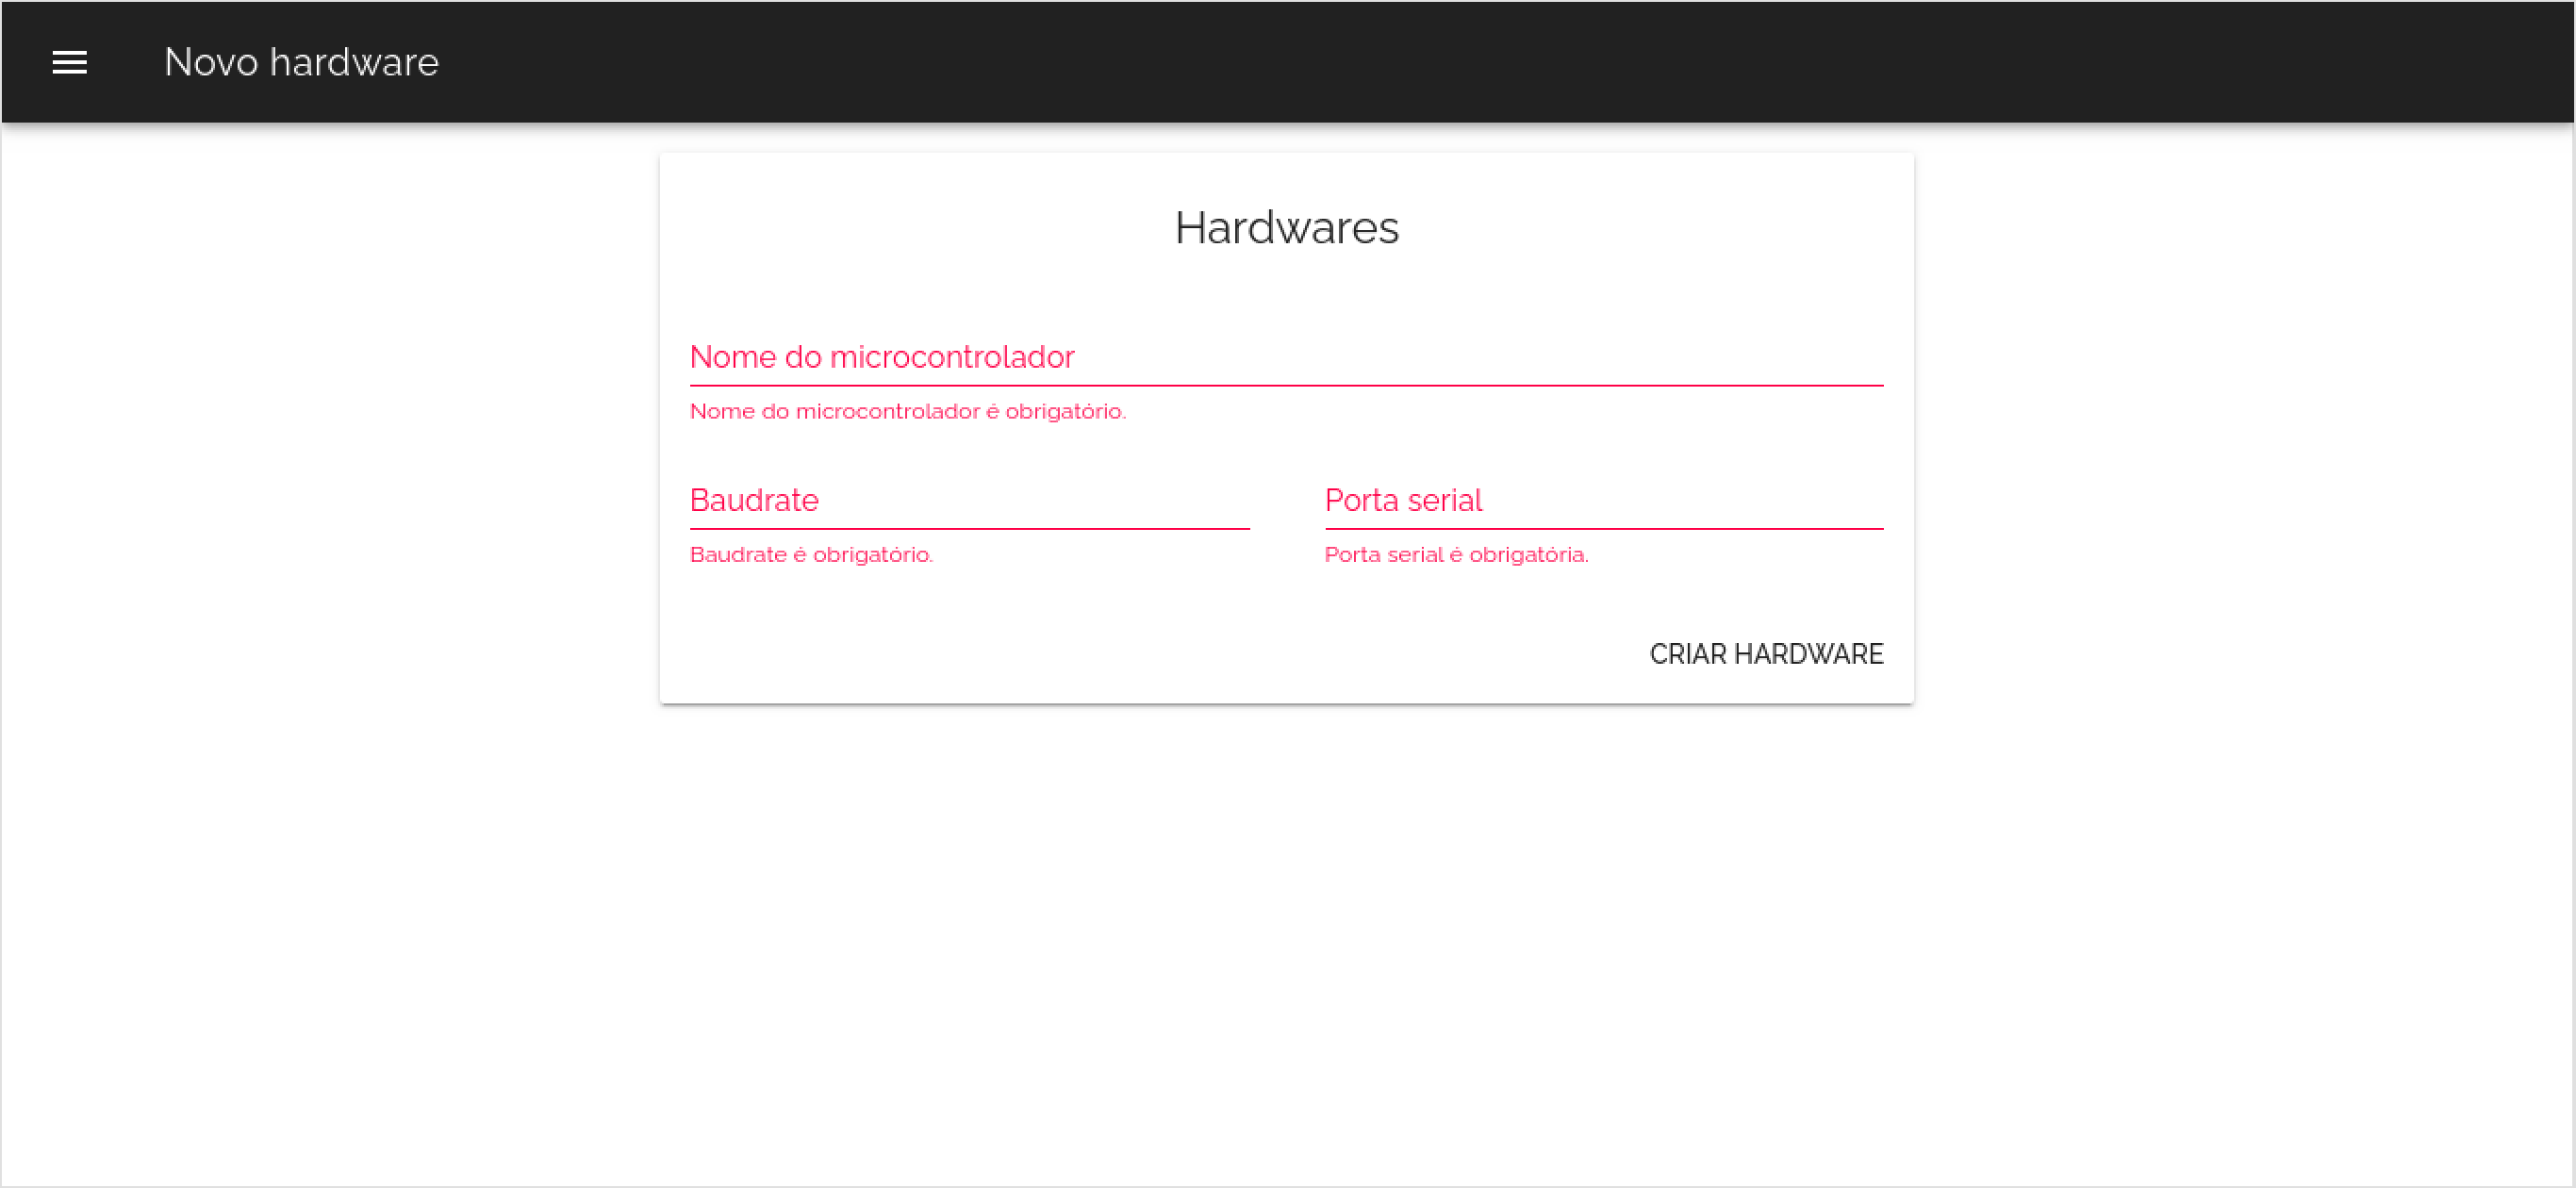
\includegraphics[width=\textwidth]{Figuras/telas/2-error.png}
        \label{teladehardware}
	\caption{ Tela de inserção de hardware}
\end{figure} 
\end{center}


A partir do menu, comandos também podem ser adicionados a partir da Figura \ref{teladecomando}. 
\begin{center}
\begin{figure}[H]					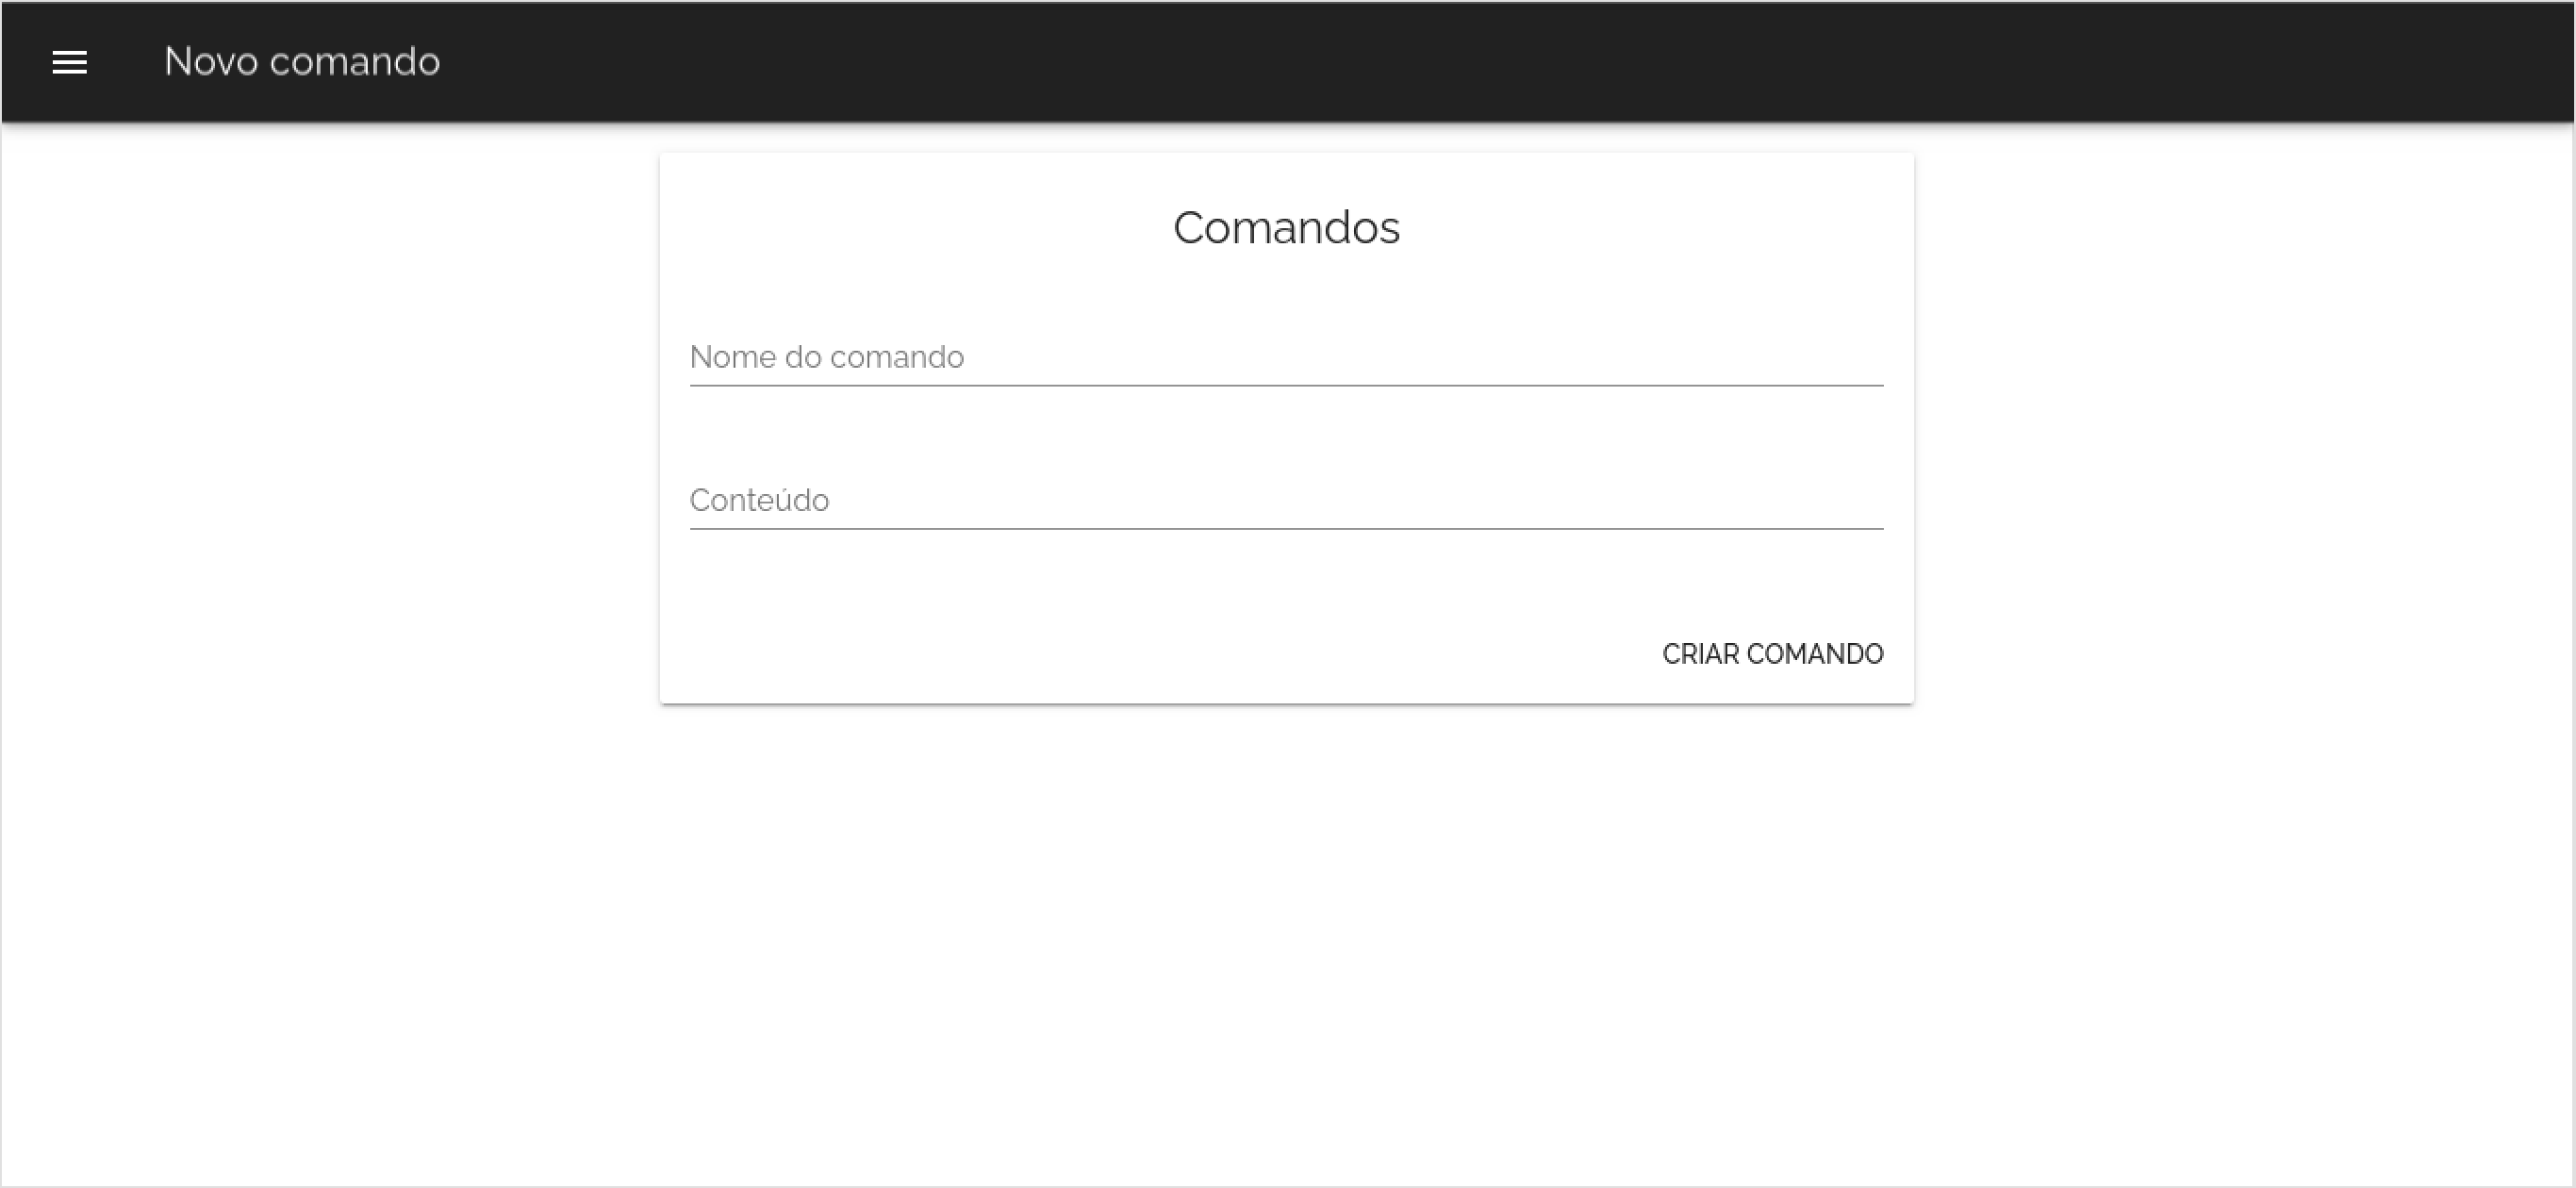
\includegraphics[width=\textwidth]{Figuras/telas/3.png}
        \label{teladecomando}
	\caption{Tela de novo comando}
\end{figure} 
\end{center}

Como pode-se observar na Figura \ref{telanovamissao}, para cadastrar uma nova missão selecione a opção Nova missão e preencha os dados conforme indicado. Após isso, clique em 'pŕóximo' para ir para a Figura \ref{telainiciarmissao} e selecionar qual foguete deseja designar para a missão.
\begin{center}
    

\begin{figure}[H]					
\includegraphics[width=\textwidth]{Figuras/telas/4.png}
        \label{telanovamissao}
	\caption{ Tela de nova missão}
\end{figure} 
\end{center}


\begin{center}
    

\begin{figure}[H]					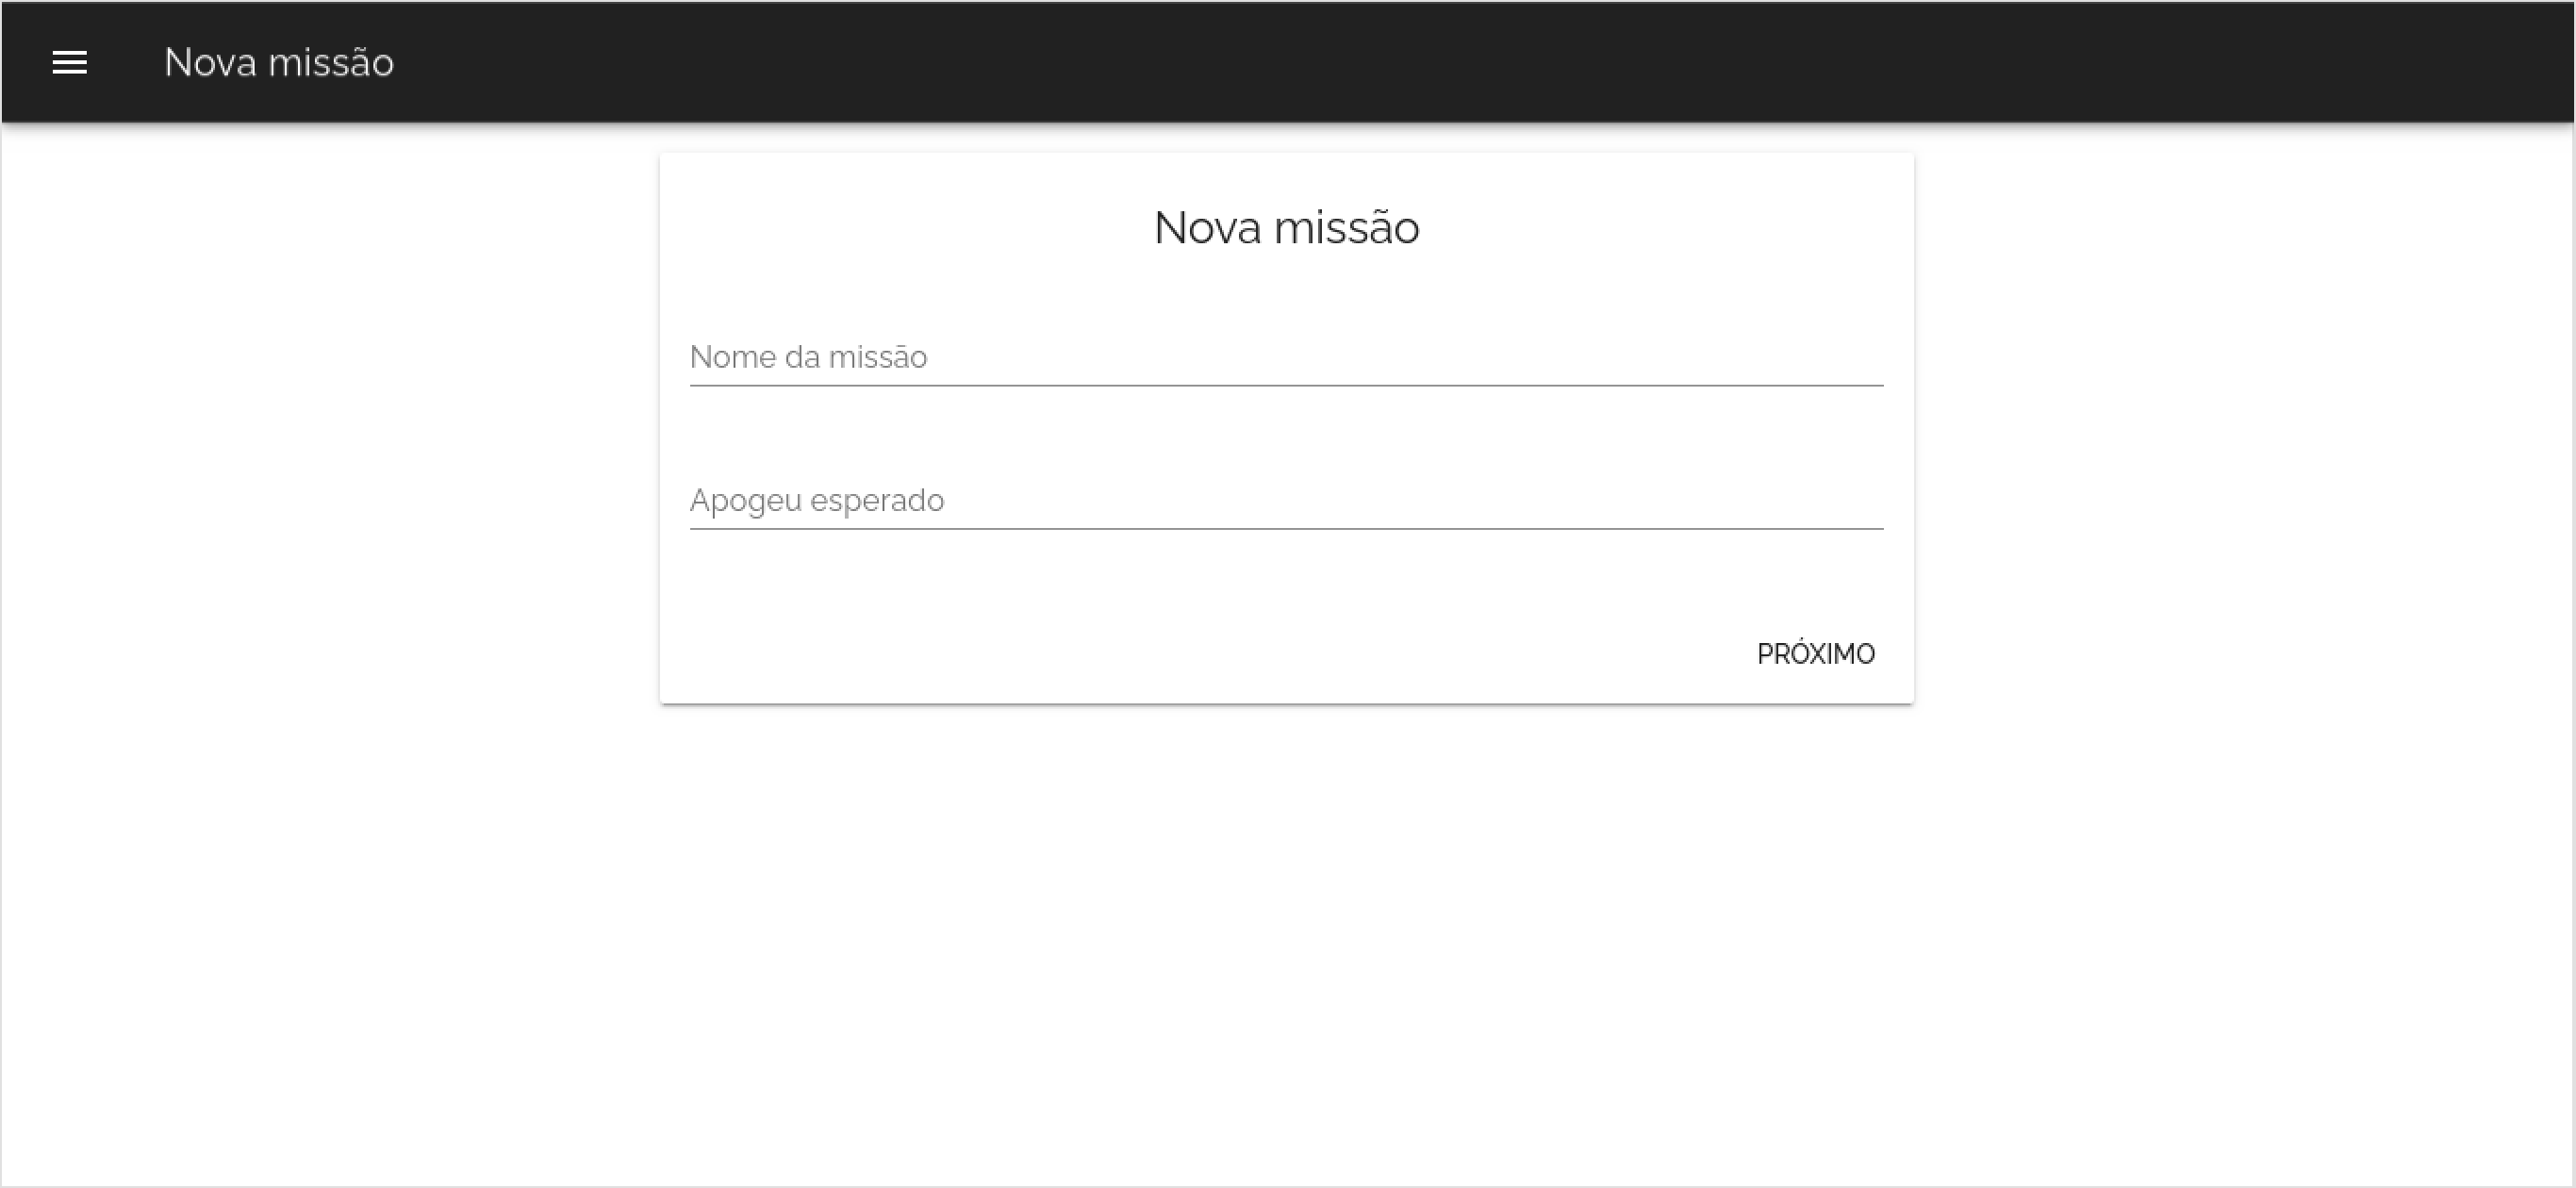
\includegraphics[width=\textwidth]{Figuras/telas/5.png}
        \label{telainiciarmissao}
	\caption{ Tela de iniciar missão}
\end{figure} 
\end{center}
\chapter{Cuidados com os equipamentos}

\begin{center}
    \begin{figure}[H]
    \centering
		
\includegraphics[scale=1.6]{Figuras/bateria/iconeimportante.png}
	    \label{iconeimportante}
    \end{figure} 
  
    	Informação importante sobre \textbf{CUIDADOS COM OS EQUIPAMENTOS}
 \end{center} 

\subsubsection*{Manuseio da PCB e componentes eletrônicos}

\PAR É de bom grado ter alguns cuidados para manter em boas condições as placas de circuito impresso-PCI que estão sujeitas a vários fatores de risco como:
\begin{itemize}
\item \textbf{Mecânicos:}
\begin{itemize}
\item Vibrações
\item flexões nas PCI 
\item choques mecânicos
\end{itemize}
\end{itemize}

\begin{itemize}
\item \textbf{Ambientais:}
\begin{itemize}
\item Umidade em excesso
\item Contaminantes pelo ar 
\item Excesso de luz solar
\end{itemize}
\end{itemize}

\begin{itemize}
\item \textbf{Eletrostático:}
\begin{itemize}
\item Descargas elétricas produzidas por atrito e contato humano sem devidos cuidados
\end{itemize}
\end{itemize}

\par {\textbf{Alguns cuidados devem ser tomados:}}

\begin{itemize}
\item Evitar tocar em partes metálicas dos componentes e nos conectores e minimizar o manuseio o máximo possível evitando danos mecânicos;
\item É recomendável segurar a placa de forma a não tocar nas suas trilhas preferível que o manuseamento da mesma seja feito de forma que a pessoa segura a placa pelas suas bordas/ laterais;  
\item Nunca flexione a placa ou utilize de muita força ao manuseá-la pode acarretar em rompimento das trilhas,rompimentos de ligações  de encaixe;
\item Nunca molhe a placa de circuito impresso e evite que a mesma entre em contato com ambientes muito úmidos e ser exposta por muito tempo a luz solar;
\end{itemize}

\subsubsection*{Manuseio das superfícies estruturais}

\par A seguir são apresentados os cuidados que deve-se ter com o equipamento estrutural do produto. Leia com atenção para preservar a vida útil do seu equipamento.

\begin{itemize}
    \item Não exponha as maletas a fumaça intensa ou gases, para não danificar o exterior do produto.
    \item Não armazene ou transporte o líquidos propelente dentro das maletas, por ser potencialmente explosivo.
    \item Mantenha as maletas e cases secas, umidade e líquidos podem danificar o revestimento ou infiltrar nas paredes estruturais.
    \item Não aplique cargas de tração nas maletas, elas não foram projetadas para isso.
    \item Não aplique cargas dinâmicas nas maletas, elas não foram projetadas para isso. E podem entrar em ressonância.
    \item Por possuir exterior emborrachado e estrutura de madeira o sistema é inflamável, não submeta-o a altas temperaturas ou ao fogo.
    \item Não cause impactos na estrutura.
    \item Não torça ou deforme o produto.
    \item É de bom grado que o usuário não sente, ou suba nas maletas estruturais.
    \item Não desmonte, modifique ou conserte as maletas sem supervisão de um técnico qualificado para este fim.
    \item Não utilize objetos pontiagudos, líquidos inflamáveis ou limpadores abrasivos.
    \item Não exponha sua estrutura de PLA a acetona, pois ela ira derreter.
    \item A borracha externa pode quebrar em ambientes de baixa umidade, mantenha sua estrutura sempre hidratada.
\end{itemize}

\chapter{Limpeza e Manutenção}

\section*{Sistema eletroeletrônico}
\par Para a limpeza e manutenção dos componentes eletrônicos e placas de circuito impresso recomendasse a utilização de Álcool Isopropílico para a sua limpeza por possuir a miníma ou nenhuma porcentagem de água evitando a oxidação dos componentes e trilhas das placas e pincel antiestática para assegura o pleno funcionamento das placas com o decorrer do tempo. Para limpeza é necessário os seguintes materiais: 
\begin{itemize}
    \item Álcool Isopropílico
    \item Pinça
    \item Algodão
    \item Pincel antiestática
\end{itemize}

\par Passos:
\begin{itemize}
    \item Limpe as placas de circuito impresso com cuidado e passando o pincel antiestática sobre todo comprimento da placa como na figura \ref{fig:pincel} para a remoção da camada de partículas sobre a placa.
    \begin{figure}[H]
  \centering
  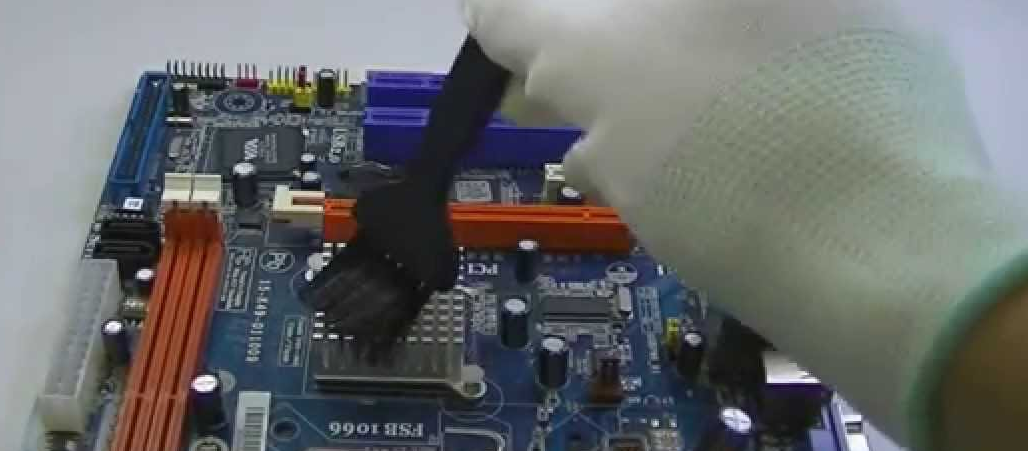
\includegraphics[width=\textwidth]{Figuras/pincel.png}
  \caption{Limpeza com pincel.} 
  \label{fig:pincel}
\end{figure}
\item Para a limpeza é necessário pegar um pedaço de algodão com a pinça e colocar Álcool Isopropílico nele, limpar as conexões de solda e as tarinhas de maneira cuidadosa evitado danos a placa. 
    \begin{figure}[H]
  \centering
  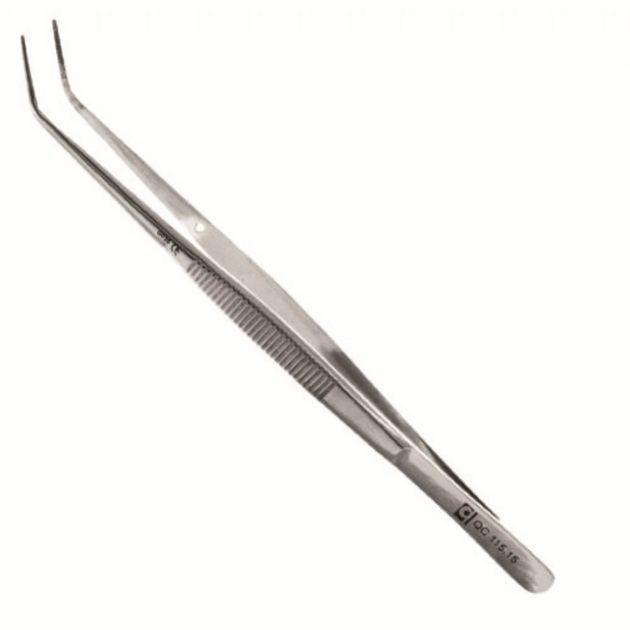
\includegraphics[scale=0.2]{Figuras/Pinca-para-Algodao-Quinelato.jpg}
    
\includegraphics[scale=0.3]{Figuras/alcool-500ml-1-90045.jpg}
      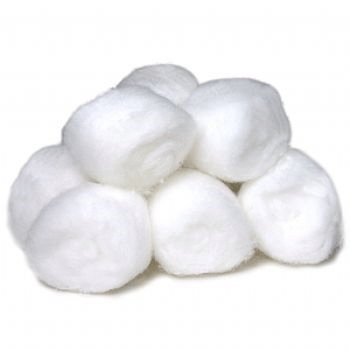
\includegraphics[scale=0.3]{Figuras/Bolas-de-Algodao.png}
  \caption{Limpeza com Álcool Isopropílico.} 
  \label{fig:alcoo}
\end{figure}

    \end{itemize}

\section*{Sistema hidráulico}

\par As partes do sistema de abastecimento que entrarem em contato com o propelente líquido, devem ser ao final do uso, expostas ao ar ambiente para entrar em contato com o oxigênio e evaporar os resquícios que possam existir ainda dentro do sistema. 

\par As válvulas e mangueiras utilizadas, não devem entrar em contato com outras substâncias que não sejam as indicadas, para o uso do sistema. Porém caso aconteça da tubulação entrar em contato com alguma substância externa, recomenda-se o uso de um pano macio e sem fiapos levemente umidificado e bem torcido, ou o auxilio de hastes de algodão para a limpeza interna.

\subsection*{Sistema de atuação}

\par O sistema de atuação é feito de uma case da aço SAE 1020, por isso para limpar o mesmo deve-se seguir as recomendações de limpeza e conservação de aço carbono. Assim a limpeza deve ser feita com um pano úmido, sabão neutro e esponja de nylon. Pelo fato do sistema possuir um motor dentro dele não é recomendado a lavagem da case em contato direto com a água por causa dos riscos de danificação do sistema. Após a limpeza seque bem a parte externa com um pano macio, seco e limpo, além de garantir que toda a umidade foi eliminada, pois aço carbono corre o risco de corroer caso não fique bem seco.

\par Deve-se atentar ao fato de que a válvula esfera é presa por dois mancais dentro da estrutura de atuação, e os mesmos devem ser lubrificados periodicamente de acordo com as especificações do fabricante.

\section*{Estrutura}

\par A seguir são apresentadas algumas dicas gerais para a limpeza e manutenção do seu produto.

\begin{itemize}
    \item Não utilize materiais de limpeza inflamáveis ou tóxicos, a não ser quando recomendado.
    \item Não faça qualquer manutenção ou limpeza no produto com ele conectado a rede elétrica ou com as baterias carregadas.
    \item Limpe as partes interiores usando um pano macio ou hastes de algodão de preferência.
    \item Se a estrutura for exposta a algum tipo de substância líquida ou química, limpe-o com um pano macio e sem fiapos.
\end{itemize}

\subsection*{Partes em MDF}

\par A estrutura das maletas são feitas em MDF, porém apesar de seu exterior revestido, seu interior ainda está sujeito ao contato com o ambiente externo. Por isso para limpar o interior do mesmo alguns cuidados devem ser seguidos, primeiramente o MDF cru não deve entrar em contato com a água, pois sua composição não é hidrofóbica.

\par Sabendo-se disso deve-se seguir as recomendações de limpeza apresentadas, onde a limpeza deve ser feita com um pano úmido e bem torcido, caso aja manchas na superfície pode-se usar uma substância a base de álcool ou sabão neutro para a limpeza. Se necessário seque com um pano seco e limpo.

\subsection*{Partes Emborrachadas}

\par A limpeza de materiais emborrachados, segue as mesmas diretrizes apresentadas anteriormente para o MDF, atentando-se ao fato de que não é recomendado o uso de álcool para a limpeza deste. Para uma secagem adequada recomenda-se deixar a estrutura ao ar livre até a secagem por completo do material. 

\par Borrachas são sensíveis a mudanças ambientais e podem ressecar e quebrar com o tempo, para que isso não ocorra é recomendado o uso de uma solução hidratante para borrachas que deve ser aplicada ao menos duas vezes ao ano.

\subsection*{Partes em PLA}

\par O PLA é um tipo de plástico desenvolvido para a impressão 3D, por isso para sua limpeza deve-se tomar as medidas de limpeza de um plástico comum. De forma que a limpeza do mesmo pode ser feita usando-se um pano úmido e sabão neutro, caso necessário pode-se fazer uso de uma esponja domestica para tirar manchas e sujeiras. 

\par Está também não deve entrar em contato direto com a água para não danificar as PCI's que comportam.

\par O PLA é um material solúvel a acetona então é muito importante para a integridade da estrutura que ela não seja exposta a esta substância.
%\chapter{Problemas e soluções}
\chapter{Informações complementares}

\section*{Uso e manuseio do Óxido Nitroso}

\begin{center}
ATENÇÃO
    \begin{figure}[H]
\centering

\includegraphics[scale = 0.1]{Figuras/atenção.png}
\end{figure}
\end{center}

\par O Óxido Nitroso é um gás não tóxico e não irritante com um efeito anestésico moderado e pode ser inalado misturado com oxigênio ou ar. Quando inalado sem oxigênio age como um asfixiante simples. No Brasil a Norma Regulamentadora 15 (NR 15), considera o produto como asfixiante simples e não impõe limites de exposição, entretanto, deve-se garantir que a concentração mínima de oxigênio seja de 18\% em volume. 

\par O sistema não vem com o cilindro de óxido nitroso, porém entende-se que o usuário que adquirir o produto estará lidando com esse tipo de propelente. Dessa forma para a segurança do cliente e correto manuseio de todas as partes do sistema indica-se a leitura dos protocolos de segurança estabelecidos para o uso e manuseio do óxido nitroso. Como fonte de referencia indica-se o seguinte \href{https://www.airliquidehealthcare.com.br/sites/alh_br/files/23003_oxido_nitroso_liquido_refrigerado10024-97-2.pdf}{link} de leitura.

\section*{Documentação técnica}

\par O seguinte produto é de desenvolvimento educacional, com caráter pre-eliminar e de prototipagem. Sua documentação técnica e de desenvolvimento encontram-se disponíveis para acesso através do repositório desenvolvido pelo grupo. 

\par Todas as informações encontram-se devidamente documentadas no relatório de desenvolvimento e seus aspectos de construção detalhados em seu manual de montagem.

\par É proibida a produção e venda deste sem autorização dos direitos intelectuais por parte do grupo desenvolvedor.

\section*{Descarte correto do equipamento}

    \begin{figure}[H]
    \centering
		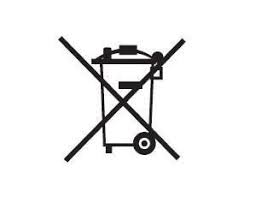
\includegraphics[scale=1]{Figuras/lixo.jpg}
    \end{figure} 
    
\par Resíduos de equipamentos Elétricos e Eletrônicos não deverão ser descartados juntamente com os resíduos domésticos. Assim como as baterias não devem ser descartadas com o lixo doméstico no final de sua vida útil. Isso se dá para impedir danos ao ambiente ou à saúde pública causados pelo descarte indevido de resíduos. Dessa forma você deverá separar estes equipamentos de outros tipos de resíduos e reciclá-los de forma responsável, de modo a promover uma reutilização sustentável dos recursos materiais.
\begin{center}
A equipe desenvolvedora apoia o seguinte movimento:
     \begin{figure}[H]
    \centering
		
\includegraphics[scale=0.5]{Figuras/lixo_eletronico.jpg}
    \end{figure} 
\end{center}

\chapter{Garantia}

\par O seu produto RGS é garantido contra defeitos de fabricação, pelo
prazo de 12 meses, contado a partir da data da emissão da Nota Fiscal ou da entrega do produto, ao primeiro adquirente.

\par A garantia compreende a substituição de peças e mão-de-obra no reparo de defeitos devidamente constatados, pelo fabricante como sendo de fabricação.

\section*{A garantia fica automaticamente invalidada se:}

\begin{itemize}
\item O produto for usado de forma indevida ou para uma destinação ao qual não foi projetado;
\item Durante a utilização do produto não forem seguidas as instruções do manual de usuário;
\item Durante a montagem do sistema as instruções de montagem e instalação não forem seguidas de acordo com o manual.
\item O usuário tenha feito um uso inadequado do produto ou alterações não autorizadas pelo fabricante.
\end{itemize}


\section*{A garantia não cobre:}

\begin{itemize}
\item Falhas do produto decorrentes de insuficiência de energia elétrica.
\item Falhas no funcionamento normal do produto decorrentes da falta de limpeza.
\item Produtos ou peças que tenham sido danificados em consequência de manuseio errado ou quedas por partes do usuário.
\item Falhas decorrentes de forças da natureza.
\end{itemize}






\end{document}
